\documentclass[a4paper]{book}
\usepackage{makeidx}
\usepackage{natbib}
\usepackage{graphicx}
\usepackage{multicol}
\usepackage{float}
\usepackage{listings}
\usepackage{color}
\usepackage{ifthen}
\usepackage[table]{xcolor}
\usepackage{textcomp}
\usepackage{alltt}
\usepackage{ifpdf}
\ifpdf
\usepackage[pdftex,
            pagebackref=true,
            colorlinks=true,
            linkcolor=blue,
            unicode
           ]{hyperref}
\else
\usepackage[ps2pdf,
            pagebackref=true,
            colorlinks=true,
            linkcolor=blue,
            unicode
           ]{hyperref}
\usepackage{pspicture}
\fi
\usepackage[utf8]{inputenc}
\usepackage{mathptmx}
\usepackage[scaled=.90]{helvet}
\usepackage{courier}
\usepackage{sectsty}
\usepackage[titles]{tocloft}
\usepackage{doxygen}
\lstset{language=C++,inputencoding=utf8,basicstyle=\footnotesize,breaklines=true,breakatwhitespace=true,tabsize=8,numbers=left }
\makeindex
\setcounter{tocdepth}{3}
\renewcommand{\footrulewidth}{0.4pt}
\renewcommand{\familydefault}{\sfdefault}
\hfuzz=15pt
\setlength{\emergencystretch}{15pt}
\hbadness=750
\tolerance=750
\begin{document}
\hypersetup{pageanchor=false,citecolor=blue}
\begin{titlepage}
\vspace*{7cm}
\begin{center}
{\Large \-Racing \\[1ex]\large 0.\-0.\-1 }\\
\vspace*{1cm}
{\large \-Generated by Doxygen 1.7.5.1}\\
\vspace*{0.5cm}
{\small Mon Sep 5 2011 20:42:38}\\
\end{center}
\end{titlepage}
\clearemptydoublepage
\pagenumbering{roman}
\tableofcontents
\clearemptydoublepage
\pagenumbering{arabic}
\hypersetup{pageanchor=true,citecolor=blue}
\chapter{\-Class \-Index}
\section{\-Class \-Hierarchy}
\-This inheritance list is sorted roughly, but not completely, alphabetically\-:\begin{DoxyCompactList}
\item \contentsline{section}{\-Matrix}{\pageref{class_matrix}}{}
\begin{DoxyCompactList}
\item \contentsline{section}{\-Matrix4f}{\pageref{class_matrix4f}}{}
\begin{DoxyCompactList}
\item \contentsline{section}{\-Camera}{\pageref{class_camera}}{}
\item \contentsline{section}{\-Frustum}{\pageref{class_frustum}}{}
\end{DoxyCompactList}
\end{DoxyCompactList}
\item \contentsline{section}{\-Model}{\pageref{class_model}}{}
\item \contentsline{section}{shader\-Resources}{\pageref{structshader_resources}}{}
\item \contentsline{section}{\-Vector}{\pageref{class_vector}}{}
\end{DoxyCompactList}

\chapter{\-Class \-Index}
\section{\-Class \-List}
\-Here are the classes, structs, unions and interfaces with brief descriptions\-:\begin{DoxyCompactList}
\item\contentsline{section}{\hyperlink{class_camera}{\-Camera} }{\pageref{class_camera}}{}
\item\contentsline{section}{\hyperlink{class_frustum}{\-Frustum} }{\pageref{class_frustum}}{}
\item\contentsline{section}{\hyperlink{class_matrix}{\-Matrix} }{\pageref{class_matrix}}{}
\item\contentsline{section}{\hyperlink{class_matrix4f}{\-Matrix4f} }{\pageref{class_matrix4f}}{}
\item\contentsline{section}{\hyperlink{class_model}{\-Model} }{\pageref{class_model}}{}
\item\contentsline{section}{\hyperlink{structshader_resources}{shader\-Resources} }{\pageref{structshader_resources}}{}
\item\contentsline{section}{\hyperlink{class_vector}{\-Vector} }{\pageref{class_vector}}{}
\end{DoxyCompactList}

\chapter{\-File \-Index}
\section{\-File \-List}
\-Here is a list of all files with brief descriptions\-:\begin{DoxyCompactList}
\item\contentsline{section}{\-Source/\hyperlink{3dmath_8cpp}{3dmath.\-cpp} }{\pageref{3dmath_8cpp}}{}
\item\contentsline{section}{\-Source/\hyperlink{3dmath_8h}{3dmath.\-h} }{\pageref{3dmath_8h}}{}
\item\contentsline{section}{\-Source/\hyperlink{_camera_8cpp}{\-Camera.\-cpp} }{\pageref{_camera_8cpp}}{}
\item\contentsline{section}{\-Source/\hyperlink{_camera_8h}{\-Camera.\-h} }{\pageref{_camera_8h}}{}
\item\contentsline{section}{\-Source/\hyperlink{_frustum_8cpp}{\-Frustum.\-cpp} }{\pageref{_frustum_8cpp}}{}
\item\contentsline{section}{\-Source/\hyperlink{_frustum_8h}{\-Frustum.\-h} }{\pageref{_frustum_8h}}{}
\item\contentsline{section}{\-Source/\hyperlink{_graphics_8cpp}{\-Graphics.\-cpp} }{\pageref{_graphics_8cpp}}{}
\item\contentsline{section}{\-Source/\hyperlink{_graphics_8h}{\-Graphics.\-h} }{\pageref{_graphics_8h}}{}
\item\contentsline{section}{\-Source/\hyperlink{main_8cpp}{main.\-cpp} }{\pageref{main_8cpp}}{}
\item\contentsline{section}{\-Source/\hyperlink{_matrix_8cpp}{\-Matrix.\-cpp} }{\pageref{_matrix_8cpp}}{}
\item\contentsline{section}{\-Source/\hyperlink{_matrix_8h}{\-Matrix.\-h} }{\pageref{_matrix_8h}}{}
\item\contentsline{section}{\-Source/\hyperlink{_matrix4f_8cpp}{\-Matrix4f.\-cpp} }{\pageref{_matrix4f_8cpp}}{}
\item\contentsline{section}{\-Source/\hyperlink{_matrix4f_8h}{\-Matrix4f.\-h} }{\pageref{_matrix4f_8h}}{}
\item\contentsline{section}{\-Source/\hyperlink{_model_8cpp}{\-Model.\-cpp} }{\pageref{_model_8cpp}}{}
\item\contentsline{section}{\-Source/\hyperlink{_model_8h}{\-Model.\-h} }{\pageref{_model_8h}}{}
\item\contentsline{section}{\-Source/\hyperlink{_vector_8cpp}{\-Vector.\-cpp} }{\pageref{_vector_8cpp}}{}
\item\contentsline{section}{\-Source/\hyperlink{_vector_8h}{\-Vector.\-h} }{\pageref{_vector_8h}}{}
\end{DoxyCompactList}

\chapter{\-Class \-Documentation}
\hypertarget{class_camera}{
\section{\-Camera \-Class \-Reference}
\label{class_camera}\index{\-Camera@{\-Camera}}
}


{\ttfamily \#include $<$\-Camera.\-h$>$}

\-Inheritance diagram for \-Camera\-:\begin{figure}[H]
\begin{center}
\leavevmode
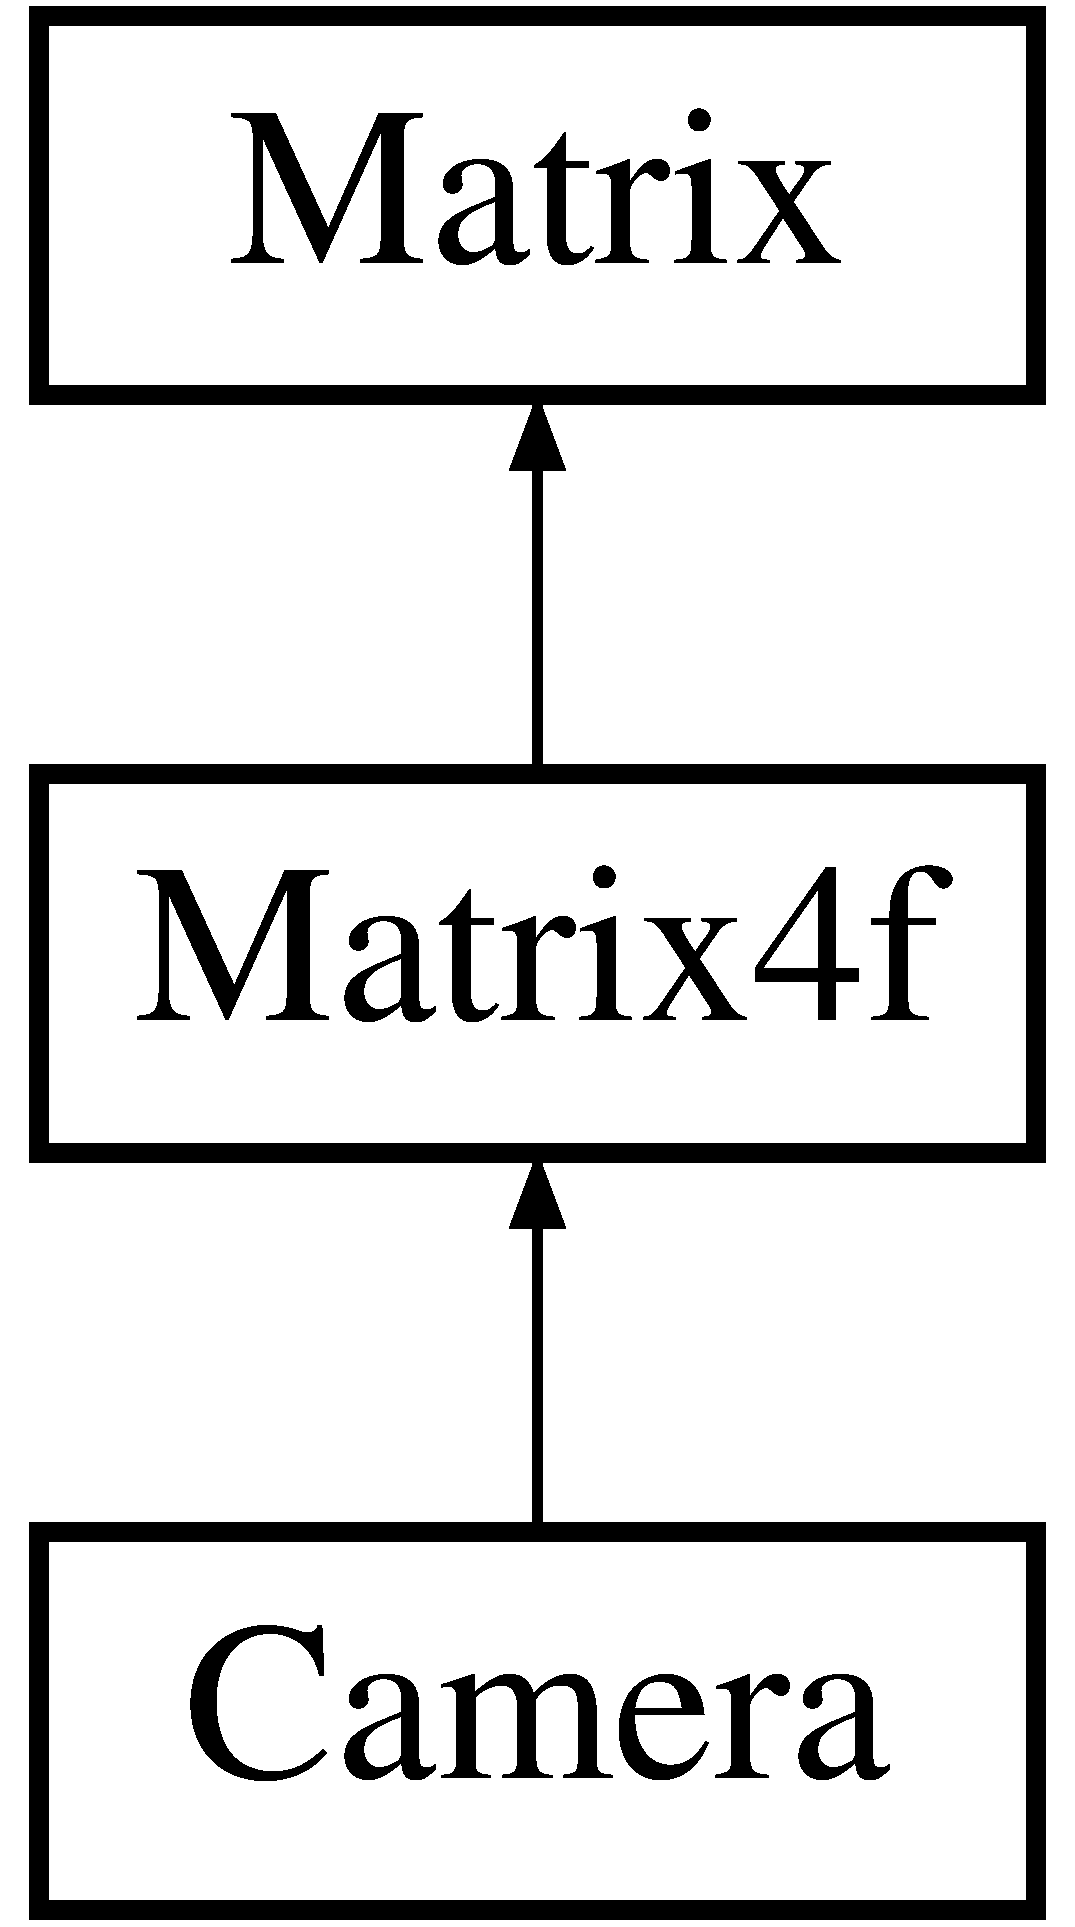
\includegraphics[height=3.000000cm]{class_camera}
\end{center}
\end{figure}
\subsection*{\-Public \-Member \-Functions}
\begin{DoxyCompactItemize}
\item 
\hyperlink{class_camera_a01f94c3543f56ede7af49dc778f19331}{\-Camera} ()
\item 
void \hyperlink{class_camera_a72e9bbc76218e616198cb600ea2723b7}{move\-Foward} (\-G\-Lfloat foward)
\item 
void \hyperlink{class_camera_a0e6065d7ba67c36a1ac63896d4a566e5}{move\-Right} (\-G\-Lfloat right)
\item 
void \hyperlink{class_camera_aed6269acf13e7aee9b0b3e8e475f5fd8}{move\-Up} (\-G\-Lfloat up)
\end{DoxyCompactItemize}


\subsection{\-Detailed \-Description}
\-A camera class. \-A camera used to control and alter the view of the user. 

\subsection{\-Constructor \& \-Destructor \-Documentation}
\hypertarget{class_camera_a01f94c3543f56ede7af49dc778f19331}{
\index{\-Camera@{\-Camera}!\-Camera@{\-Camera}}
\index{\-Camera@{\-Camera}!Camera@{\-Camera}}
\subsubsection[{\-Camera}]{\setlength{\rightskip}{0pt plus 5cm}\-Camera\-::\-Camera (
\begin{DoxyParamCaption}
{}
\end{DoxyParamCaption}
)\hspace{0.3cm}{\ttfamily  \mbox{[}inline\mbox{]}}}}
\label{class_camera_a01f94c3543f56ede7af49dc778f19331}
\-A constructor. \-The constructor set the camera matrix to an identity matrix 

\subsection{\-Member \-Function \-Documentation}
\hypertarget{class_camera_a72e9bbc76218e616198cb600ea2723b7}{
\index{\-Camera@{\-Camera}!move\-Foward@{move\-Foward}}
\index{move\-Foward@{move\-Foward}!Camera@{\-Camera}}
\subsubsection[{move\-Foward}]{\setlength{\rightskip}{0pt plus 5cm}void \-Camera\-::move\-Foward (
\begin{DoxyParamCaption}
\item[{\-G\-Lfloat}]{foward}
\end{DoxyParamCaption}
)\hspace{0.3cm}{\ttfamily  \mbox{[}inline\mbox{]}}}}
\label{class_camera_a72e9bbc76218e616198cb600ea2723b7}
moves the camera forward. 
\begin{DoxyParams}{\-Parameters}
{\em foward} & a \-G\-Lfloat representing the amount to move the camera forward can be negative to move the camera back. \\
\hline
\end{DoxyParams}
\hypertarget{class_camera_a0e6065d7ba67c36a1ac63896d4a566e5}{
\index{\-Camera@{\-Camera}!move\-Right@{move\-Right}}
\index{move\-Right@{move\-Right}!Camera@{\-Camera}}
\subsubsection[{move\-Right}]{\setlength{\rightskip}{0pt plus 5cm}void \-Camera\-::move\-Right (
\begin{DoxyParamCaption}
\item[{\-G\-Lfloat}]{right}
\end{DoxyParamCaption}
)\hspace{0.3cm}{\ttfamily  \mbox{[}inline\mbox{]}}}}
\label{class_camera_a0e6065d7ba67c36a1ac63896d4a566e5}
moves the camera right. 
\begin{DoxyParams}{\-Parameters}
{\em right} & a \-G\-Lfloat representing the amount to move the camera right can be negative to move the camera left. \\
\hline
\end{DoxyParams}
\hypertarget{class_camera_aed6269acf13e7aee9b0b3e8e475f5fd8}{
\index{\-Camera@{\-Camera}!move\-Up@{move\-Up}}
\index{move\-Up@{move\-Up}!Camera@{\-Camera}}
\subsubsection[{move\-Up}]{\setlength{\rightskip}{0pt plus 5cm}void \-Camera\-::move\-Up (
\begin{DoxyParamCaption}
\item[{\-G\-Lfloat}]{up}
\end{DoxyParamCaption}
)\hspace{0.3cm}{\ttfamily  \mbox{[}inline\mbox{]}}}}
\label{class_camera_aed6269acf13e7aee9b0b3e8e475f5fd8}
moves the camera up. 
\begin{DoxyParams}{\-Parameters}
{\em up} & a \-G\-Lfloat representing the amount to move the camera up can be negative to move the camera down. \\
\hline
\end{DoxyParams}


\-The documentation for this class was generated from the following file\-:\begin{DoxyCompactItemize}
\item 
\-Source/\hyperlink{_camera_8h}{\-Camera.\-h}\end{DoxyCompactItemize}

\hypertarget{class_frustum}{
\section{\-Frustum \-Class \-Reference}
\label{class_frustum}\index{\-Frustum@{\-Frustum}}
}


{\ttfamily \#include $<$\-Frustum.\-h$>$}

\-Inheritance diagram for \-Frustum\-:\begin{figure}[H]
\begin{center}
\leavevmode
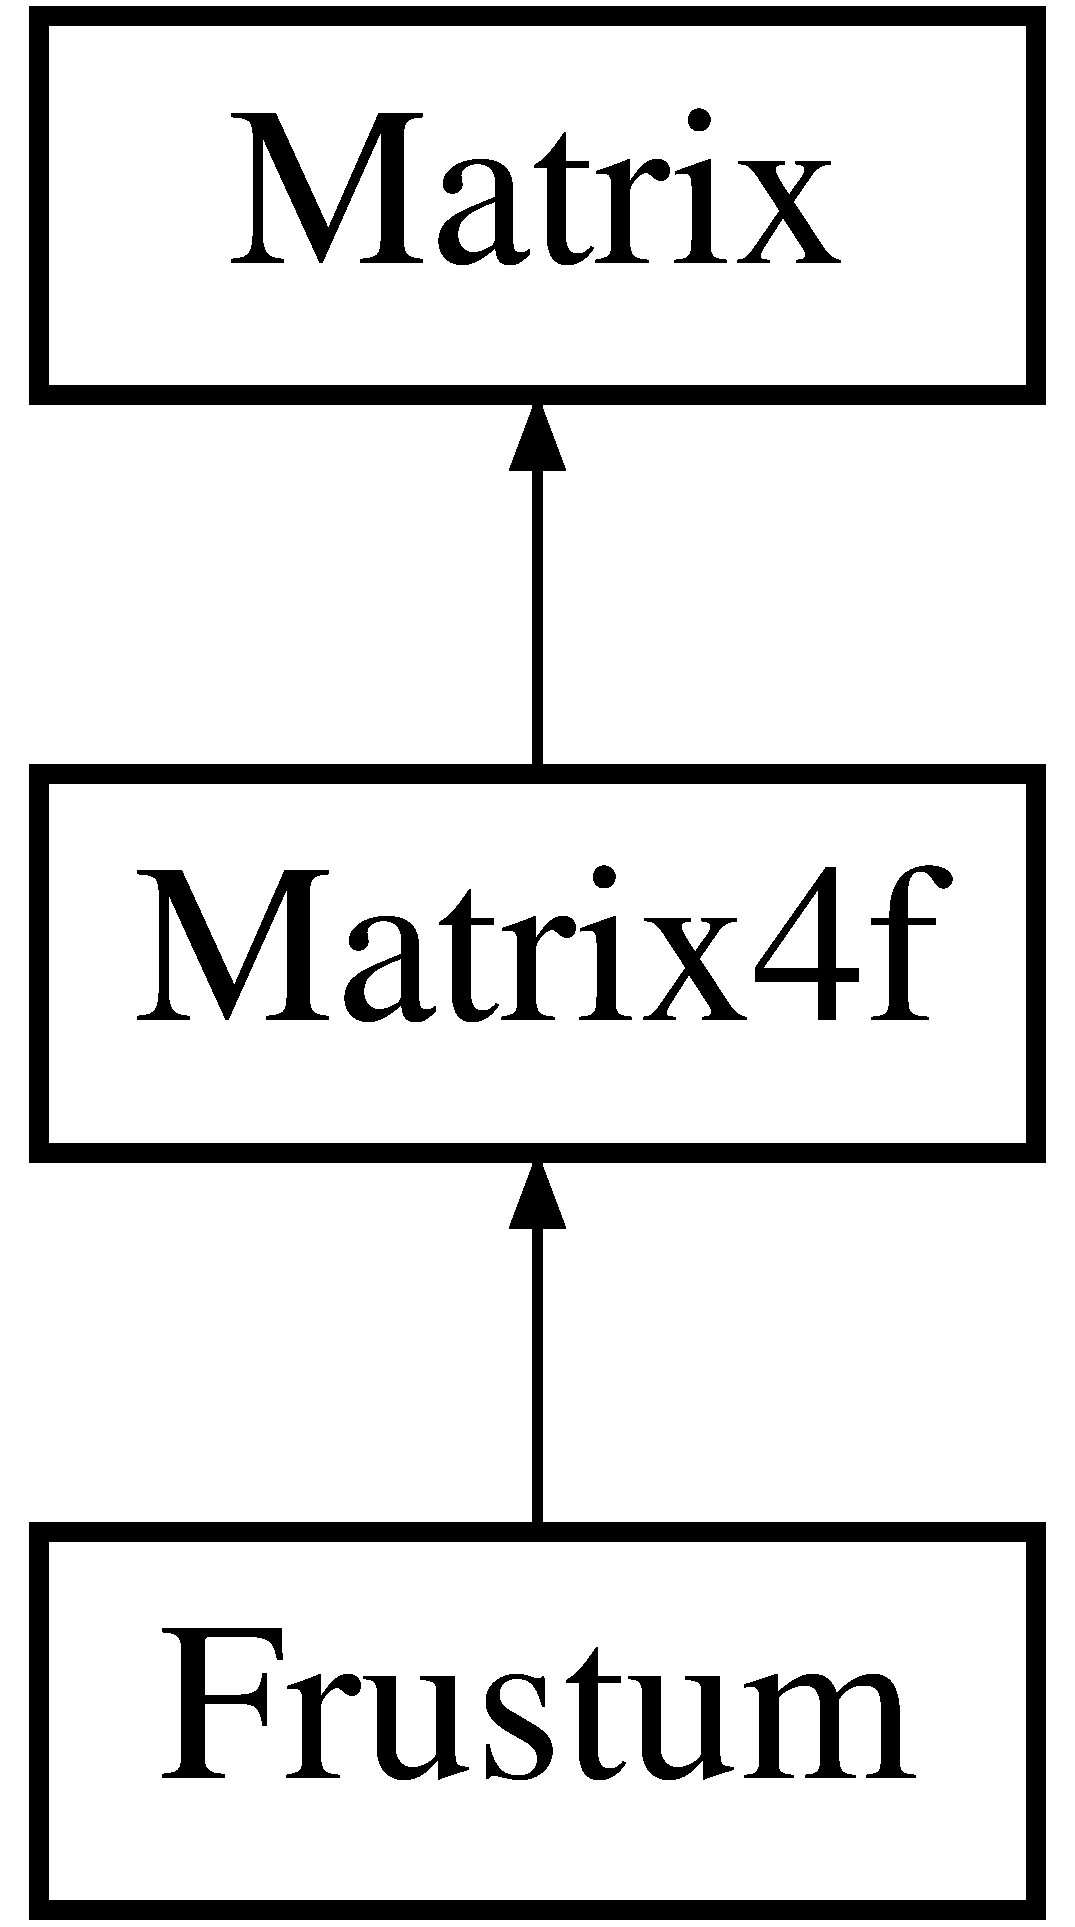
\includegraphics[height=3.000000cm]{class_frustum}
\end{center}
\end{figure}
\subsection*{\-Public \-Member \-Functions}
\begin{DoxyCompactItemize}
\item 
\hyperlink{class_frustum_a172ae3492592e3ac891642299d628494}{\-Frustum} ()
\item 
void \hyperlink{class_frustum_a0a046fcea2667b5e5541154a410c99ef}{set\-Perspective} (\-G\-Lfloat aspect, \-G\-Lfloat angle, \-G\-Lfloat near, \-G\-Lfloat far)
\end{DoxyCompactItemize}


\subsection{\-Detailed \-Description}
\-A \-Frustrum class. 

\subsection{\-Constructor \& \-Destructor \-Documentation}
\hypertarget{class_frustum_a172ae3492592e3ac891642299d628494}{
\index{\-Frustum@{\-Frustum}!\-Frustum@{\-Frustum}}
\index{\-Frustum@{\-Frustum}!Frustum@{\-Frustum}}
\subsubsection[{\-Frustum}]{\setlength{\rightskip}{0pt plus 5cm}\-Frustum\-::\-Frustum (
\begin{DoxyParamCaption}
{}
\end{DoxyParamCaption}
)\hspace{0.3cm}{\ttfamily  \mbox{[}inline\mbox{]}}}}
\label{class_frustum_a172ae3492592e3ac891642299d628494}
\-A constructor. \-Sets the frustum to an identity matrix. 

\subsection{\-Member \-Function \-Documentation}
\hypertarget{class_frustum_a0a046fcea2667b5e5541154a410c99ef}{
\index{\-Frustum@{\-Frustum}!set\-Perspective@{set\-Perspective}}
\index{set\-Perspective@{set\-Perspective}!Frustum@{\-Frustum}}
\subsubsection[{set\-Perspective}]{\setlength{\rightskip}{0pt plus 5cm}void \-Frustum\-::set\-Perspective (
\begin{DoxyParamCaption}
\item[{\-G\-Lfloat}]{aspect, }
\item[{\-G\-Lfloat}]{angle, }
\item[{\-G\-Lfloat}]{near, }
\item[{\-G\-Lfloat}]{far}
\end{DoxyParamCaption}
)\hspace{0.3cm}{\ttfamily  \mbox{[}inline\mbox{]}}}}
\label{class_frustum_a0a046fcea2667b5e5541154a410c99ef}
set\-Perspective sets the orientation of the frustrum 
\begin{DoxyParams}{\-Parameters}
{\em aspect} & a \-G\-Lfloat that sets the aspect ratio of the frustum \\
\hline
{\em angle} & a \-G\-Lfloat that sets the viewing angle of the frustum \\
\hline
{\em near} & a \-G\-Lfloat that sets the near value of the frustum \\
\hline
{\em far} & a \-G\-Lfloat that sets the far value of the frustum \\
\hline
\end{DoxyParams}


\-The documentation for this class was generated from the following files\-:\begin{DoxyCompactItemize}
\item 
\-Source/\hyperlink{_frustum_8h}{\-Frustum.\-h}\item 
\-Source/\hyperlink{_frustum_8cpp}{\-Frustum.\-cpp}\end{DoxyCompactItemize}

\hypertarget{class_matrix}{
\section{\-Matrix \-Class \-Reference}
\label{class_matrix}\index{\-Matrix@{\-Matrix}}
}


{\ttfamily \#include $<$\-Matrix.\-h$>$}

\-Inheritance diagram for \-Matrix\-:\begin{figure}[H]
\begin{center}
\leavevmode
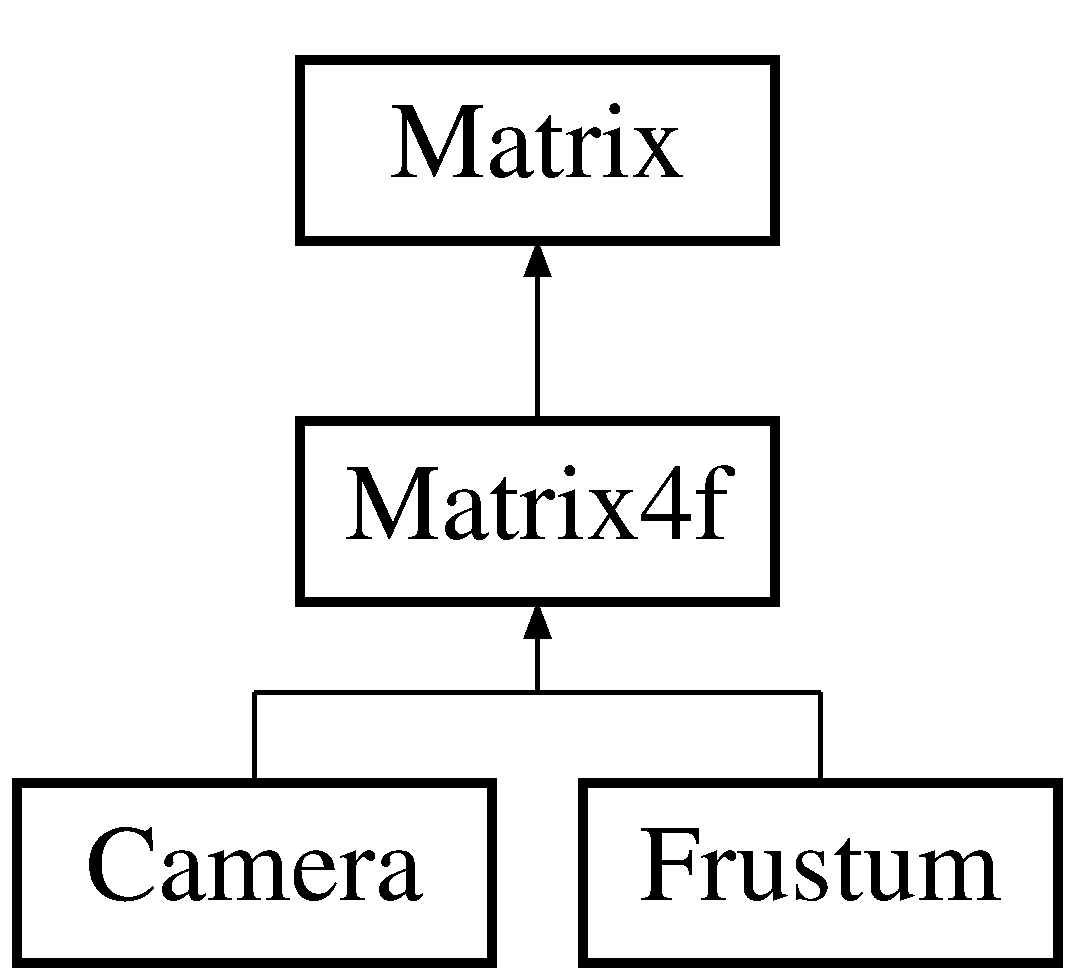
\includegraphics[height=3.000000cm]{class_matrix}
\end{center}
\end{figure}
\subsection*{\-Public \-Member \-Functions}
\begin{DoxyCompactItemize}
\item 
\hyperlink{class_matrix_ad38857ddffc21c51fcf626e284e7282f}{\-Matrix} (int \hyperlink{class_matrix_ad4320bd2dc03fd11887d3ba350c6c8ef}{width}, int \hyperlink{class_matrix_a0b5614256a04ece0ea54b8aad7e6980c}{height}, std\-::vector$<$ \-G\-Lfloat $>$ v)
\item 
\hyperlink{class_matrix_ab19b1c231dedb3ab0b11af42e9aa7ef4}{\-Matrix} (\hyperlink{class_matrix}{\-Matrix} const \&other)
\item 
void \hyperlink{class_matrix_a130e415b12d0a0c338d8d0961131bc3e}{operator=} (const \hyperlink{class_matrix}{\-Matrix} \&rhs)
\item 
\hyperlink{class_matrix}{\-Matrix} \& \hyperlink{class_matrix_ab25d7df6ae0a248aa220b6191f56961a}{operator$\ast$=} (const \hyperlink{class_matrix}{\-Matrix} \&rhs)
\item 
const \hyperlink{class_matrix}{\-Matrix} \hyperlink{class_matrix_a6e1a01475e178191c70a488bb7316903}{operator$\ast$} (const \hyperlink{class_matrix}{\-Matrix} \&rhs) const 
\item 
const \-G\-Lfloat \hyperlink{class_matrix_a19a5cc379e90bc99e6dcee1f8a79dfb1}{operator\mbox{[}$\,$\mbox{]}} (const int n) const 
\item 
int \hyperlink{class_matrix_a3b8788a3ed5bbc00cea54d4be60ef786}{get\-Width} () const 
\item 
int \hyperlink{class_matrix_a2c8ede48d107858a2308a6c530135eed}{get\-Height} () const 
\end{DoxyCompactItemize}
\subsection*{\-Protected \-Attributes}
\begin{DoxyCompactItemize}
\item 
int \hyperlink{class_matrix_ad4320bd2dc03fd11887d3ba350c6c8ef}{width}
\item 
int \hyperlink{class_matrix_a0b5614256a04ece0ea54b8aad7e6980c}{height}
\item 
std\-::vector$<$ \-G\-Lfloat $>$ \hyperlink{class_matrix_a7b0bacf179e0b5ac7d5e74b7eff9e353}{values}
\end{DoxyCompactItemize}


\subsection{\-Detailed \-Description}
\-A matrix class. \-A matrix that is stored column major. 

\subsection{\-Constructor \& \-Destructor \-Documentation}
\hypertarget{class_matrix_ad38857ddffc21c51fcf626e284e7282f}{
\index{\-Matrix@{\-Matrix}!\-Matrix@{\-Matrix}}
\index{\-Matrix@{\-Matrix}!Matrix@{\-Matrix}}
\subsubsection[{\-Matrix}]{\setlength{\rightskip}{0pt plus 5cm}\-Matrix\-::\-Matrix (
\begin{DoxyParamCaption}
\item[{int}]{width, }
\item[{int}]{height, }
\item[{std\-::vector$<$ \-G\-Lfloat $>$}]{v}
\end{DoxyParamCaption}
)}}
\label{class_matrix_ad38857ddffc21c51fcf626e284e7282f}
\-A constructor. 
\begin{DoxyParams}{\-Parameters}
{\em width} & an int the width of the matrix \\
\hline
{\em height} & an int the height of the matrix \\
\hline
{\em v} & a vector$<$\-G\-Lfloat$>$ the contents of the matrix \\
\hline
\end{DoxyParams}
\hypertarget{class_matrix_ab19b1c231dedb3ab0b11af42e9aa7ef4}{
\index{\-Matrix@{\-Matrix}!\-Matrix@{\-Matrix}}
\index{\-Matrix@{\-Matrix}!Matrix@{\-Matrix}}
\subsubsection[{\-Matrix}]{\setlength{\rightskip}{0pt plus 5cm}\-Matrix\-::\-Matrix (
\begin{DoxyParamCaption}
\item[{{\bf \-Matrix} const \&}]{other}
\end{DoxyParamCaption}
)}}
\label{class_matrix_ab19b1c231dedb3ab0b11af42e9aa7ef4}
\-A copy constructor. 
\begin{DoxyParams}{\-Parameters}
{\em other} & the other matrix to copy \\
\hline
\end{DoxyParams}


\subsection{\-Member \-Function \-Documentation}
\hypertarget{class_matrix_a2c8ede48d107858a2308a6c530135eed}{
\index{\-Matrix@{\-Matrix}!get\-Height@{get\-Height}}
\index{get\-Height@{get\-Height}!Matrix@{\-Matrix}}
\subsubsection[{get\-Height}]{\setlength{\rightskip}{0pt plus 5cm}int \-Matrix\-::get\-Height (
\begin{DoxyParamCaption}
{}
\end{DoxyParamCaption}
) const\hspace{0.3cm}{\ttfamily  \mbox{[}inline\mbox{]}}}}
\label{class_matrix_a2c8ede48d107858a2308a6c530135eed}
get\-Height returns the height \begin{DoxyReturn}{\-Returns}
the height of the matrix as an int 
\end{DoxyReturn}
\hypertarget{class_matrix_a3b8788a3ed5bbc00cea54d4be60ef786}{
\index{\-Matrix@{\-Matrix}!get\-Width@{get\-Width}}
\index{get\-Width@{get\-Width}!Matrix@{\-Matrix}}
\subsubsection[{get\-Width}]{\setlength{\rightskip}{0pt plus 5cm}int \-Matrix\-::get\-Width (
\begin{DoxyParamCaption}
{}
\end{DoxyParamCaption}
) const\hspace{0.3cm}{\ttfamily  \mbox{[}inline\mbox{]}}}}
\label{class_matrix_a3b8788a3ed5bbc00cea54d4be60ef786}
get\-Width returns the width \begin{DoxyReturn}{\-Returns}
the width of the matrix as an int 
\end{DoxyReturn}
\hypertarget{class_matrix_a6e1a01475e178191c70a488bb7316903}{
\index{\-Matrix@{\-Matrix}!operator$\ast$@{operator$\ast$}}
\index{operator$\ast$@{operator$\ast$}!Matrix@{\-Matrix}}
\subsubsection[{operator$\ast$}]{\setlength{\rightskip}{0pt plus 5cm}const {\bf \-Matrix} \-Matrix\-::operator$\ast$ (
\begin{DoxyParamCaption}
\item[{const {\bf \-Matrix} \&}]{rhs}
\end{DoxyParamCaption}
) const}}
\label{class_matrix_a6e1a01475e178191c70a488bb7316903}
overloads the $\ast$ operator 
\begin{DoxyParams}{\-Parameters}
{\em rhs} & the other matrix to multiply by. \\
\hline
\end{DoxyParams}
\begin{DoxyReturn}{\-Returns}
returns a constant matrix created by multiplying this by rhs 
\end{DoxyReturn}
\hypertarget{class_matrix_ab25d7df6ae0a248aa220b6191f56961a}{
\index{\-Matrix@{\-Matrix}!operator$\ast$=@{operator$\ast$=}}
\index{operator$\ast$=@{operator$\ast$=}!Matrix@{\-Matrix}}
\subsubsection[{operator$\ast$=}]{\setlength{\rightskip}{0pt plus 5cm}{\bf \-Matrix} \& \-Matrix\-::operator$\ast$= (
\begin{DoxyParamCaption}
\item[{const {\bf \-Matrix} \&}]{rhs}
\end{DoxyParamCaption}
)}}
\label{class_matrix_ab25d7df6ae0a248aa220b6191f56961a}
overloads the $\ast$= operator. 
\begin{DoxyParams}{\-Parameters}
{\em rhs} & the other matrix to multiply by \\
\hline
\end{DoxyParams}
\begin{DoxyReturn}{\-Returns}
returns this matrix 
\end{DoxyReturn}
\hypertarget{class_matrix_a130e415b12d0a0c338d8d0961131bc3e}{
\index{\-Matrix@{\-Matrix}!operator=@{operator=}}
\index{operator=@{operator=}!Matrix@{\-Matrix}}
\subsubsection[{operator=}]{\setlength{\rightskip}{0pt plus 5cm}void \-Matrix\-::operator= (
\begin{DoxyParamCaption}
\item[{const {\bf \-Matrix} \&}]{rhs}
\end{DoxyParamCaption}
)}}
\label{class_matrix_a130e415b12d0a0c338d8d0961131bc3e}
overloads the = operator. 
\begin{DoxyParams}{\-Parameters}
{\em rhs} & the other matrix to copy \\
\hline
\end{DoxyParams}


\-Reimplemented in \hyperlink{class_matrix4f_a8e06b155b8ee0414bf46103dc4d66856}{\-Matrix4f}.

\hypertarget{class_matrix_a19a5cc379e90bc99e6dcee1f8a79dfb1}{
\index{\-Matrix@{\-Matrix}!operator\mbox{[}$\,$\mbox{]}@{operator[]}}
\index{operator\mbox{[}$\,$\mbox{]}@{operator[]}!Matrix@{\-Matrix}}
\subsubsection[{operator[]}]{\setlength{\rightskip}{0pt plus 5cm}const \-G\-Lfloat \-Matrix\-::operator\mbox{[}$\,$\mbox{]} (
\begin{DoxyParamCaption}
\item[{const int}]{n}
\end{DoxyParamCaption}
) const}}
\label{class_matrix_a19a5cc379e90bc99e6dcee1f8a79dfb1}
overloads the \mbox{[}\mbox{]} operator. 
\begin{DoxyParams}{\-Parameters}
{\em n} & as an int representing the index \\
\hline
\end{DoxyParams}
\begin{DoxyReturn}{\-Returns}
the nth element 
\end{DoxyReturn}


\subsection{\-Member \-Data \-Documentation}
\hypertarget{class_matrix_a0b5614256a04ece0ea54b8aad7e6980c}{
\index{\-Matrix@{\-Matrix}!height@{height}}
\index{height@{height}!Matrix@{\-Matrix}}
\subsubsection[{height}]{\setlength{\rightskip}{0pt plus 5cm}int {\bf \-Matrix\-::height}\hspace{0.3cm}{\ttfamily  \mbox{[}protected\mbox{]}}}}
\label{class_matrix_a0b5614256a04ece0ea54b8aad7e6980c}
\hypertarget{class_matrix_a7b0bacf179e0b5ac7d5e74b7eff9e353}{
\index{\-Matrix@{\-Matrix}!values@{values}}
\index{values@{values}!Matrix@{\-Matrix}}
\subsubsection[{values}]{\setlength{\rightskip}{0pt plus 5cm}std\-::vector$<$\-G\-Lfloat$>$ {\bf \-Matrix\-::values}\hspace{0.3cm}{\ttfamily  \mbox{[}protected\mbox{]}}}}
\label{class_matrix_a7b0bacf179e0b5ac7d5e74b7eff9e353}
\hypertarget{class_matrix_ad4320bd2dc03fd11887d3ba350c6c8ef}{
\index{\-Matrix@{\-Matrix}!width@{width}}
\index{width@{width}!Matrix@{\-Matrix}}
\subsubsection[{width}]{\setlength{\rightskip}{0pt plus 5cm}int {\bf \-Matrix\-::width}\hspace{0.3cm}{\ttfamily  \mbox{[}protected\mbox{]}}}}
\label{class_matrix_ad4320bd2dc03fd11887d3ba350c6c8ef}


\-The documentation for this class was generated from the following files\-:\begin{DoxyCompactItemize}
\item 
\-Source/\hyperlink{_matrix_8h}{\-Matrix.\-h}\item 
\-Source/\hyperlink{_matrix_8cpp}{\-Matrix.\-cpp}\end{DoxyCompactItemize}

\hypertarget{class_matrix4f}{
\section{\-Matrix4f \-Class \-Reference}
\label{class_matrix4f}\index{\-Matrix4f@{\-Matrix4f}}
}


{\ttfamily \#include $<$\-Matrix4f.\-h$>$}

\-Inheritance diagram for \-Matrix4f\-:\begin{figure}[H]
\begin{center}
\leavevmode
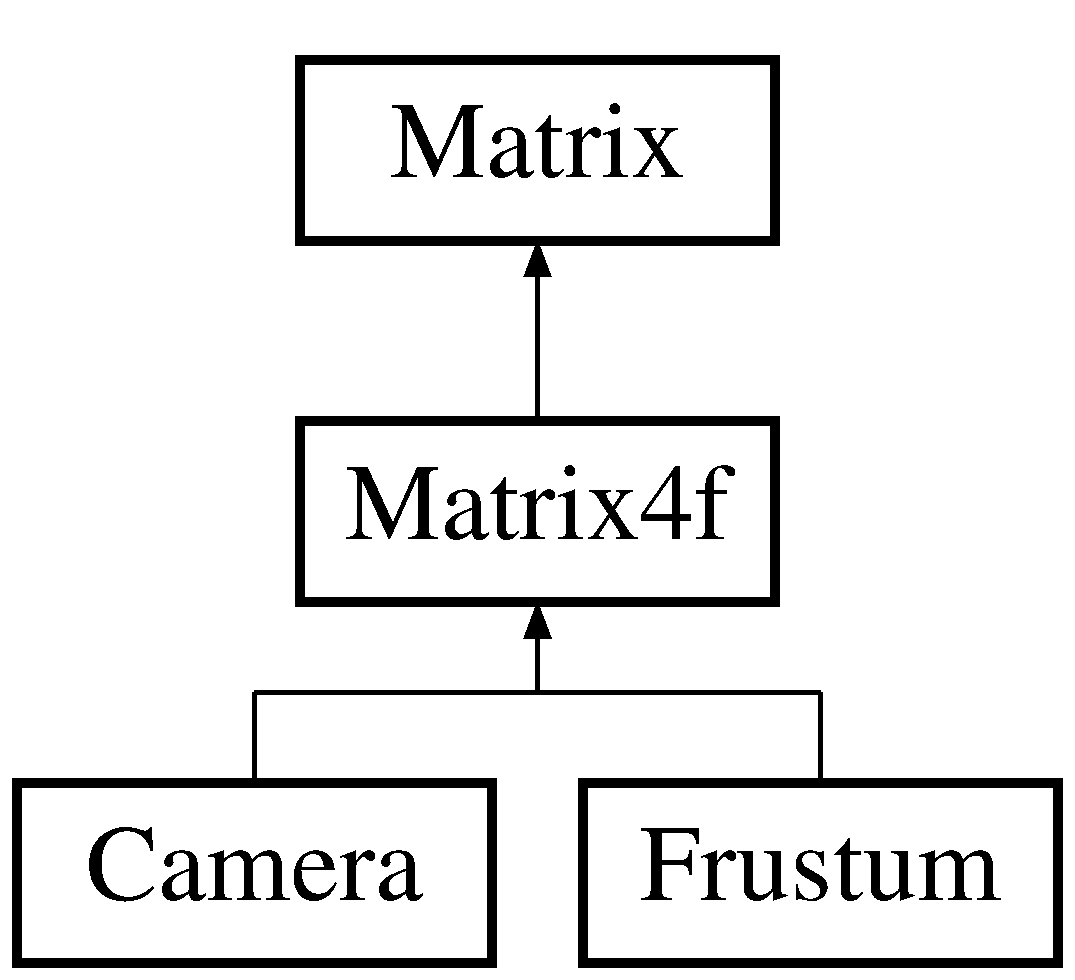
\includegraphics[height=3.000000cm]{class_matrix4f}
\end{center}
\end{figure}
\subsection*{\-Public \-Member \-Functions}
\begin{DoxyCompactItemize}
\item 
\hyperlink{class_matrix4f}{\-Matrix4f} \hyperlink{class_matrix4f_a8e06b155b8ee0414bf46103dc4d66856}{operator=} (const \hyperlink{class_matrix}{\-Matrix} \&rhs)
\item 
\hyperlink{class_matrix4f_a2aea81514a71d644a97d8d0b3971a858}{\-Matrix4f} ()
\item 
\hyperlink{class_matrix4f_ae52bef2ab502a173e03fdd6913a215e5}{\-Matrix4f} (std\-::vector$<$ \-G\-Lfloat $>$ \hyperlink{class_matrix_a7b0bacf179e0b5ac7d5e74b7eff9e353}{values})
\item 
\hyperlink{class_matrix4f}{\-Matrix4f} \hyperlink{class_matrix4f_ab5601849252dfee2b0a3475b1620b545}{rotate} (\-G\-Lfloat x, \-G\-Lfloat y, \-G\-Lfloat z)
\item 
\hyperlink{class_matrix4f}{\-Matrix4f} \hyperlink{class_matrix4f_a63e0c8b1c4a13bb98de2b85af70b300b}{translate} (\-G\-Lfloat x, \-G\-Lfloat y, \-G\-Lfloat z)
\item 
\hyperlink{class_matrix4f}{\-Matrix4f} \hyperlink{class_matrix4f_aa6b9fbf059fef2d6807a14940f8c2915}{scale} (\-G\-Lfloat x, \-G\-Lfloat y, \-G\-Lfloat z)
\item 
void \hyperlink{class_matrix4f_ac76d8eddcf58efbcb08148c883717498}{load\-Uniform} (\-G\-Lint loc)
\end{DoxyCompactItemize}


\subsection{\-Detailed \-Description}
\hyperlink{class_matrix4f}{\-Matrix4f} a 4x4 matrix class. 

\subsection{\-Constructor \& \-Destructor \-Documentation}
\hypertarget{class_matrix4f_a2aea81514a71d644a97d8d0b3971a858}{
\index{\-Matrix4f@{\-Matrix4f}!\-Matrix4f@{\-Matrix4f}}
\index{\-Matrix4f@{\-Matrix4f}!Matrix4f@{\-Matrix4f}}
\subsubsection[{\-Matrix4f}]{\setlength{\rightskip}{0pt plus 5cm}\-Matrix4f\-::\-Matrix4f (
\begin{DoxyParamCaption}
{}
\end{DoxyParamCaption}
)\hspace{0.3cm}{\ttfamily  \mbox{[}inline\mbox{]}}}}
\label{class_matrix4f_a2aea81514a71d644a97d8d0b3971a858}
\-A constructor that sets this matrix to the identity matrix. \hypertarget{class_matrix4f_ae52bef2ab502a173e03fdd6913a215e5}{
\index{\-Matrix4f@{\-Matrix4f}!\-Matrix4f@{\-Matrix4f}}
\index{\-Matrix4f@{\-Matrix4f}!Matrix4f@{\-Matrix4f}}
\subsubsection[{\-Matrix4f}]{\setlength{\rightskip}{0pt plus 5cm}\-Matrix4f\-::\-Matrix4f (
\begin{DoxyParamCaption}
\item[{std\-::vector$<$ \-G\-Lfloat $>$}]{values}
\end{DoxyParamCaption}
)\hspace{0.3cm}{\ttfamily  \mbox{[}inline\mbox{]}}}}
\label{class_matrix4f_ae52bef2ab502a173e03fdd6913a215e5}
\-A constructor that sets this matrix to values. 
\begin{DoxyParams}{\-Parameters}
{\em values} & a 16 element vector$<$\-G\-Lfloat$>$ representing the values to set this matrix to. \\
\hline
\end{DoxyParams}


\subsection{\-Member \-Function \-Documentation}
\hypertarget{class_matrix4f_ac76d8eddcf58efbcb08148c883717498}{
\index{\-Matrix4f@{\-Matrix4f}!load\-Uniform@{load\-Uniform}}
\index{load\-Uniform@{load\-Uniform}!Matrix4f@{\-Matrix4f}}
\subsubsection[{load\-Uniform}]{\setlength{\rightskip}{0pt plus 5cm}void \-Matrix4f\-::load\-Uniform (
\begin{DoxyParamCaption}
\item[{\-G\-Lint}]{loc}
\end{DoxyParamCaption}
)}}
\label{class_matrix4f_ac76d8eddcf58efbcb08148c883717498}
sends the data of this matrix as a matrixuniform. 
\begin{DoxyParams}{\-Parameters}
{\em loc} & the corresponding location. \\
\hline
\end{DoxyParams}
\hypertarget{class_matrix4f_a8e06b155b8ee0414bf46103dc4d66856}{
\index{\-Matrix4f@{\-Matrix4f}!operator=@{operator=}}
\index{operator=@{operator=}!Matrix4f@{\-Matrix4f}}
\subsubsection[{operator=}]{\setlength{\rightskip}{0pt plus 5cm}{\bf \-Matrix4f} \-Matrix4f\-::operator= (
\begin{DoxyParamCaption}
\item[{const {\bf \-Matrix} \&}]{rhs}
\end{DoxyParamCaption}
)}}
\label{class_matrix4f_a8e06b155b8ee0414bf46103dc4d66856}
overloads the = operator. 
\begin{DoxyParams}{\-Parameters}
{\em rhs} & the other matrix. \\
\hline
\end{DoxyParams}
\begin{DoxyReturn}{\-Returns}
this matrix with its new values. 
\end{DoxyReturn}


\-Reimplemented from \hyperlink{class_matrix_a130e415b12d0a0c338d8d0961131bc3e}{\-Matrix}.

\hypertarget{class_matrix4f_ab5601849252dfee2b0a3475b1620b545}{
\index{\-Matrix4f@{\-Matrix4f}!rotate@{rotate}}
\index{rotate@{rotate}!Matrix4f@{\-Matrix4f}}
\subsubsection[{rotate}]{\setlength{\rightskip}{0pt plus 5cm}{\bf \-Matrix4f} \-Matrix4f\-::rotate (
\begin{DoxyParamCaption}
\item[{\-G\-Lfloat}]{x, }
\item[{\-G\-Lfloat}]{y, }
\item[{\-G\-Lfloat}]{z}
\end{DoxyParamCaption}
)}}
\label{class_matrix4f_ab5601849252dfee2b0a3475b1620b545}
transforms this matrix by rotating it. 
\begin{DoxyParams}{\-Parameters}
{\em x} & \-G\-Lfloat the x angle to be rotated by. \\
\hline
{\em y} & \-G\-Lfloat the y angle to be rotated by. \\
\hline
{\em z} & \-G\-Lfloat the z angle to be rotated by. \\
\hline
\end{DoxyParams}
\begin{DoxyReturn}{\-Returns}
returns this newly transformed matrix. 
\end{DoxyReturn}
\hypertarget{class_matrix4f_aa6b9fbf059fef2d6807a14940f8c2915}{
\index{\-Matrix4f@{\-Matrix4f}!scale@{scale}}
\index{scale@{scale}!Matrix4f@{\-Matrix4f}}
\subsubsection[{scale}]{\setlength{\rightskip}{0pt plus 5cm}{\bf \-Matrix4f} \-Matrix4f\-::scale (
\begin{DoxyParamCaption}
\item[{\-G\-Lfloat}]{x, }
\item[{\-G\-Lfloat}]{y, }
\item[{\-G\-Lfloat}]{z}
\end{DoxyParamCaption}
)}}
\label{class_matrix4f_aa6b9fbf059fef2d6807a14940f8c2915}
transforms this matrix by scaling it. 
\begin{DoxyParams}{\-Parameters}
{\em x} & \-G\-Lfloat the x amount to be scaled by. \\
\hline
{\em y} & \-G\-Lfloat the y amount to be scaled by. \\
\hline
{\em z} & \-G\-Lfloat the z amount to be scaled by. \\
\hline
\end{DoxyParams}
\begin{DoxyReturn}{\-Returns}
returns this newly transformed matrix. 
\end{DoxyReturn}
\hypertarget{class_matrix4f_a63e0c8b1c4a13bb98de2b85af70b300b}{
\index{\-Matrix4f@{\-Matrix4f}!translate@{translate}}
\index{translate@{translate}!Matrix4f@{\-Matrix4f}}
\subsubsection[{translate}]{\setlength{\rightskip}{0pt plus 5cm}{\bf \-Matrix4f} \-Matrix4f\-::translate (
\begin{DoxyParamCaption}
\item[{\-G\-Lfloat}]{x, }
\item[{\-G\-Lfloat}]{y, }
\item[{\-G\-Lfloat}]{z}
\end{DoxyParamCaption}
)}}
\label{class_matrix4f_a63e0c8b1c4a13bb98de2b85af70b300b}
transforms this matrix by translating it. 
\begin{DoxyParams}{\-Parameters}
{\em x} & \-G\-Lfloat the x distance to be translated by. \\
\hline
{\em y} & \-G\-Lfloat the y distance to be translated by. \\
\hline
{\em z} & \-G\-Lfloat the z distance to be translated by. \\
\hline
\end{DoxyParams}
\begin{DoxyReturn}{\-Returns}
returns this newly transformed matrix. 
\end{DoxyReturn}


\-The documentation for this class was generated from the following files\-:\begin{DoxyCompactItemize}
\item 
\-Source/\hyperlink{_matrix4f_8h}{\-Matrix4f.\-h}\item 
\-Source/\hyperlink{_matrix4f_8cpp}{\-Matrix4f.\-cpp}\end{DoxyCompactItemize}

\hypertarget{class_model}{
\section{\-Model \-Class \-Reference}
\label{class_model}\index{\-Model@{\-Model}}
}


{\ttfamily \#include $<$\-Model.\-h$>$}

\subsection*{\-Public \-Member \-Functions}
\begin{DoxyCompactItemize}
\item 
\hyperlink{class_model_a2e4833699259e3cefe0e20c0eb6672e7}{\-Model} (char $\ast$filename)
\item 
void \hyperlink{class_model_a8438a257c3005fe29d2a9a6cadcac757}{draw} (\-G\-Lint pos)
\end{DoxyCompactItemize}


\subsection{\-Detailed \-Description}
\-A graphical model class. 

\subsection{\-Constructor \& \-Destructor \-Documentation}
\hypertarget{class_model_a2e4833699259e3cefe0e20c0eb6672e7}{
\index{\-Model@{\-Model}!\-Model@{\-Model}}
\index{\-Model@{\-Model}!Model@{\-Model}}
\subsubsection[{\-Model}]{\setlength{\rightskip}{0pt plus 5cm}\-Model\-::\-Model (
\begin{DoxyParamCaption}
\item[{char $\ast$}]{filename}
\end{DoxyParamCaption}
)}}
\label{class_model_a2e4833699259e3cefe0e20c0eb6672e7}
a constructor. sets the data of the model name to the information int the ogl file. 
\begin{DoxyParams}{\-Parameters}
{\em filename} & a char$\ast$ the name of the ogl file. \\
\hline
\end{DoxyParams}


\subsection{\-Member \-Function \-Documentation}
\hypertarget{class_model_a8438a257c3005fe29d2a9a6cadcac757}{
\index{\-Model@{\-Model}!draw@{draw}}
\index{draw@{draw}!Model@{\-Model}}
\subsubsection[{draw}]{\setlength{\rightskip}{0pt plus 5cm}void \-Model\-::draw (
\begin{DoxyParamCaption}
\item[{\-G\-Lint}]{pos}
\end{DoxyParamCaption}
)}}
\label{class_model_a8438a257c3005fe29d2a9a6cadcac757}
\-Draws the model. 
\begin{DoxyParams}{\-Parameters}
{\em pos} & the \-G\-Lint that corresponds to the shader vector input data. \\
\hline
\end{DoxyParams}


\-The documentation for this class was generated from the following files\-:\begin{DoxyCompactItemize}
\item 
\-Source/\hyperlink{_model_8h}{\-Model.\-h}\item 
\-Source/\hyperlink{_model_8cpp}{\-Model.\-cpp}\end{DoxyCompactItemize}

\hypertarget{structshader_resources}{
\section{shader\-Resources \-Struct \-Reference}
\label{structshader_resources}\index{shader\-Resources@{shader\-Resources}}
}
\subsection*{\-Public \-Attributes}
\begin{DoxyCompactItemize}
\item 
\-G\-Luint \hyperlink{structshader_resources_abe191bcd7c0511350d50df60d4105650}{vertex\-Shader}
\item 
\-G\-Luint \hyperlink{structshader_resources_a7f7c50ec931e8313fa125a12aec1de52}{fragment\-Shader}
\item 
\-G\-Luint \hyperlink{structshader_resources_aeb0b002a54cffa47fa0ab63402d9e877}{program}
\item 
\begin{tabbing}
xx\=xx\=xx\=xx\=xx\=xx\=xx\=xx\=xx\=\kill
struct \{\\
\>GLint \hyperlink{structshader_resources_ade284e9d31dbb5d8ae20d48ca71d4803}{colour}\\
\>GLint \hyperlink{structshader_resources_a25bf9d04069cd045b8fcd4483b25ccf5}{modelViewProjectionMatrix}\\
\} \hyperlink{structshader_resources_afa2fe5d923b03ebc556d7e139ce3d559}{uniforms}\\

\end{tabbing}\item 
\begin{tabbing}
xx\=xx\=xx\=xx\=xx\=xx\=xx\=xx\=xx\=\kill
struct \{\\
\>GLint \hyperlink{structshader_resources_a074cd8e5271a817d584c38e21a474ce2}{pos}\\
\} \hyperlink{structshader_resources_a00004b6567d1e7178a15842dd8325e42}{attributes}\\

\end{tabbing}\end{DoxyCompactItemize}


\subsection{\-Member \-Data \-Documentation}
\hypertarget{structshader_resources_a00004b6567d1e7178a15842dd8325e42}{
\index{shader\-Resources@{shader\-Resources}!attributes@{attributes}}
\index{attributes@{attributes}!shaderResources@{shader\-Resources}}
\subsubsection[{attributes}]{\setlength{\rightskip}{0pt plus 5cm}struct \{ ... \}  {\bf shader\-Resources\-::attributes}}}
\label{structshader_resources_a00004b6567d1e7178a15842dd8325e42}
\hypertarget{structshader_resources_ade284e9d31dbb5d8ae20d48ca71d4803}{
\index{shader\-Resources@{shader\-Resources}!colour@{colour}}
\index{colour@{colour}!shaderResources@{shader\-Resources}}
\subsubsection[{colour}]{\setlength{\rightskip}{0pt plus 5cm}\-G\-Lint {\bf shader\-Resources\-::colour}}}
\label{structshader_resources_ade284e9d31dbb5d8ae20d48ca71d4803}
\hypertarget{structshader_resources_a7f7c50ec931e8313fa125a12aec1de52}{
\index{shader\-Resources@{shader\-Resources}!fragment\-Shader@{fragment\-Shader}}
\index{fragment\-Shader@{fragment\-Shader}!shaderResources@{shader\-Resources}}
\subsubsection[{fragment\-Shader}]{\setlength{\rightskip}{0pt plus 5cm}\-G\-Luint {\bf shader\-Resources\-::fragment\-Shader}}}
\label{structshader_resources_a7f7c50ec931e8313fa125a12aec1de52}
\hypertarget{structshader_resources_a25bf9d04069cd045b8fcd4483b25ccf5}{
\index{shader\-Resources@{shader\-Resources}!model\-View\-Projection\-Matrix@{model\-View\-Projection\-Matrix}}
\index{model\-View\-Projection\-Matrix@{model\-View\-Projection\-Matrix}!shaderResources@{shader\-Resources}}
\subsubsection[{model\-View\-Projection\-Matrix}]{\setlength{\rightskip}{0pt plus 5cm}\-G\-Lint {\bf shader\-Resources\-::model\-View\-Projection\-Matrix}}}
\label{structshader_resources_a25bf9d04069cd045b8fcd4483b25ccf5}
\hypertarget{structshader_resources_a074cd8e5271a817d584c38e21a474ce2}{
\index{shader\-Resources@{shader\-Resources}!pos@{pos}}
\index{pos@{pos}!shaderResources@{shader\-Resources}}
\subsubsection[{pos}]{\setlength{\rightskip}{0pt plus 5cm}\-G\-Lint {\bf shader\-Resources\-::pos}}}
\label{structshader_resources_a074cd8e5271a817d584c38e21a474ce2}
\hypertarget{structshader_resources_aeb0b002a54cffa47fa0ab63402d9e877}{
\index{shader\-Resources@{shader\-Resources}!program@{program}}
\index{program@{program}!shaderResources@{shader\-Resources}}
\subsubsection[{program}]{\setlength{\rightskip}{0pt plus 5cm}\-G\-Luint {\bf shader\-Resources\-::program}}}
\label{structshader_resources_aeb0b002a54cffa47fa0ab63402d9e877}
\hypertarget{structshader_resources_afa2fe5d923b03ebc556d7e139ce3d559}{
\index{shader\-Resources@{shader\-Resources}!uniforms@{uniforms}}
\index{uniforms@{uniforms}!shaderResources@{shader\-Resources}}
\subsubsection[{uniforms}]{\setlength{\rightskip}{0pt plus 5cm}struct \{ ... \}  {\bf shader\-Resources\-::uniforms}}}
\label{structshader_resources_afa2fe5d923b03ebc556d7e139ce3d559}
\hypertarget{structshader_resources_abe191bcd7c0511350d50df60d4105650}{
\index{shader\-Resources@{shader\-Resources}!vertex\-Shader@{vertex\-Shader}}
\index{vertex\-Shader@{vertex\-Shader}!shaderResources@{shader\-Resources}}
\subsubsection[{vertex\-Shader}]{\setlength{\rightskip}{0pt plus 5cm}\-G\-Luint {\bf shader\-Resources\-::vertex\-Shader}}}
\label{structshader_resources_abe191bcd7c0511350d50df60d4105650}


\-The documentation for this struct was generated from the following file\-:\begin{DoxyCompactItemize}
\item 
\-Source/\hyperlink{main_8cpp}{main.\-cpp}\end{DoxyCompactItemize}

\hypertarget{class_vector}{
\section{\-Vector \-Class \-Reference}
\label{class_vector}\index{\-Vector@{\-Vector}}
}


{\ttfamily \#include $<$\-Vector.\-h$>$}

\subsection*{\-Public \-Member \-Functions}
\begin{DoxyCompactItemize}
\item 
\hyperlink{class_vector_a6f80c73b5f18dcf3f8e36065bdc8b9e5}{\-Vector} ()
\item 
\hyperlink{class_vector_af5311e0ef5b13bd7643355bafd9f023f}{\-Vector} (\-G\-Lfloat x, \-G\-Lfloat y, \-G\-Lfloat z, \-G\-Lfloat w=1.\-0f)
\item 
void \hyperlink{class_vector_ab1fd44956712ca844838dcf6ce76dadb}{set\-Values} (\-G\-Lfloat x, \-G\-Lfloat y, \-G\-Lfloat z, \-G\-Lfloat w=1.\-0f)
\item 
\-G\-Lfloat \hyperlink{class_vector_a520f954e0bf0cfd2ac3ba7fd9ef87b26}{get\-X} ()
\item 
\-G\-Lfloat \hyperlink{class_vector_abdc63d8dc8da39532addd27cd31ffde4}{get\-Y} ()
\item 
\-G\-Lfloat \hyperlink{class_vector_a3a5653a55fbf04c8a89daf163d2d7a87}{get\-Z} ()
\item 
\-G\-Lfloat \hyperlink{class_vector_a3653affbf6ee4f98e37b9373b11cfcd9}{get\-W} ()
\end{DoxyCompactItemize}


\subsection{\-Constructor \& \-Destructor \-Documentation}
\hypertarget{class_vector_a6f80c73b5f18dcf3f8e36065bdc8b9e5}{
\index{\-Vector@{\-Vector}!\-Vector@{\-Vector}}
\index{\-Vector@{\-Vector}!Vector@{\-Vector}}
\subsubsection[{\-Vector}]{\setlength{\rightskip}{0pt plus 5cm}\-Vector\-::\-Vector (
\begin{DoxyParamCaption}
{}
\end{DoxyParamCaption}
)}}
\label{class_vector_a6f80c73b5f18dcf3f8e36065bdc8b9e5}
\-A constructor. \hypertarget{class_vector_af5311e0ef5b13bd7643355bafd9f023f}{
\index{\-Vector@{\-Vector}!\-Vector@{\-Vector}}
\index{\-Vector@{\-Vector}!Vector@{\-Vector}}
\subsubsection[{\-Vector}]{\setlength{\rightskip}{0pt plus 5cm}\-Vector\-::\-Vector (
\begin{DoxyParamCaption}
\item[{\-G\-Lfloat}]{x, }
\item[{\-G\-Lfloat}]{y, }
\item[{\-G\-Lfloat}]{z, }
\item[{\-G\-Lfloat}]{w = {\ttfamily 1.0f}}
\end{DoxyParamCaption}
)}}
\label{class_vector_af5311e0ef5b13bd7643355bafd9f023f}
\-A constructor. 
\begin{DoxyParams}{\-Parameters}
{\em x} & \-G\-Lfloat the x value of the vector. \\
\hline
{\em y} & \-G\-Lfloat the y value of the vector. \\
\hline
{\em z} & \-G\-Lfloat the z value of the vector. \\
\hline
{\em w} & \-G\-Lfloat the w value of the vector. \\
\hline
\end{DoxyParams}


\subsection{\-Member \-Function \-Documentation}
\hypertarget{class_vector_a3653affbf6ee4f98e37b9373b11cfcd9}{
\index{\-Vector@{\-Vector}!get\-W@{get\-W}}
\index{get\-W@{get\-W}!Vector@{\-Vector}}
\subsubsection[{get\-W}]{\setlength{\rightskip}{0pt plus 5cm}\-G\-Lfloat \-Vector\-::get\-W (
\begin{DoxyParamCaption}
{}
\end{DoxyParamCaption}
)\hspace{0.3cm}{\ttfamily  \mbox{[}inline\mbox{]}}}}
\label{class_vector_a3653affbf6ee4f98e37b9373b11cfcd9}
get\-W returns the w value of the vector. \begin{DoxyReturn}{\-Returns}
returns the w value as a \-G\-Lfloat. 
\end{DoxyReturn}
\hypertarget{class_vector_a520f954e0bf0cfd2ac3ba7fd9ef87b26}{
\index{\-Vector@{\-Vector}!get\-X@{get\-X}}
\index{get\-X@{get\-X}!Vector@{\-Vector}}
\subsubsection[{get\-X}]{\setlength{\rightskip}{0pt plus 5cm}\-G\-Lfloat \-Vector\-::get\-X (
\begin{DoxyParamCaption}
{}
\end{DoxyParamCaption}
)\hspace{0.3cm}{\ttfamily  \mbox{[}inline\mbox{]}}}}
\label{class_vector_a520f954e0bf0cfd2ac3ba7fd9ef87b26}
get\-X returns the x value of the vector. \begin{DoxyReturn}{\-Returns}
returns the x value as a \-G\-Lfloat. 
\end{DoxyReturn}
\hypertarget{class_vector_abdc63d8dc8da39532addd27cd31ffde4}{
\index{\-Vector@{\-Vector}!get\-Y@{get\-Y}}
\index{get\-Y@{get\-Y}!Vector@{\-Vector}}
\subsubsection[{get\-Y}]{\setlength{\rightskip}{0pt plus 5cm}\-G\-Lfloat \-Vector\-::get\-Y (
\begin{DoxyParamCaption}
{}
\end{DoxyParamCaption}
)\hspace{0.3cm}{\ttfamily  \mbox{[}inline\mbox{]}}}}
\label{class_vector_abdc63d8dc8da39532addd27cd31ffde4}
get\-Y returns the y value of the vector. \begin{DoxyReturn}{\-Returns}
returns the y value as a \-G\-Lfloat. 
\end{DoxyReturn}
\hypertarget{class_vector_a3a5653a55fbf04c8a89daf163d2d7a87}{
\index{\-Vector@{\-Vector}!get\-Z@{get\-Z}}
\index{get\-Z@{get\-Z}!Vector@{\-Vector}}
\subsubsection[{get\-Z}]{\setlength{\rightskip}{0pt plus 5cm}\-G\-Lfloat \-Vector\-::get\-Z (
\begin{DoxyParamCaption}
{}
\end{DoxyParamCaption}
)\hspace{0.3cm}{\ttfamily  \mbox{[}inline\mbox{]}}}}
\label{class_vector_a3a5653a55fbf04c8a89daf163d2d7a87}
get\-Z returns the z value of the vector. \begin{DoxyReturn}{\-Returns}
returns the z value as a \-G\-Lfloat. 
\end{DoxyReturn}
\hypertarget{class_vector_ab1fd44956712ca844838dcf6ce76dadb}{
\index{\-Vector@{\-Vector}!set\-Values@{set\-Values}}
\index{set\-Values@{set\-Values}!Vector@{\-Vector}}
\subsubsection[{set\-Values}]{\setlength{\rightskip}{0pt plus 5cm}void \-Vector\-::set\-Values (
\begin{DoxyParamCaption}
\item[{\-G\-Lfloat}]{x, }
\item[{\-G\-Lfloat}]{y, }
\item[{\-G\-Lfloat}]{z, }
\item[{\-G\-Lfloat}]{w = {\ttfamily 1.0f}}
\end{DoxyParamCaption}
)}}
\label{class_vector_ab1fd44956712ca844838dcf6ce76dadb}
set\-Values sets the values of the vector. 
\begin{DoxyParams}{\-Parameters}
{\em x} & \-G\-Lfloat the x value of the vector. \\
\hline
{\em y} & \-G\-Lfloat the y value of the vector. \\
\hline
{\em z} & \-G\-Lfloat the z value of the vector. \\
\hline
{\em w} & \-G\-Lfloat the w value of the vector. \\
\hline
\end{DoxyParams}


\-The documentation for this class was generated from the following files\-:\begin{DoxyCompactItemize}
\item 
\-Source/\hyperlink{_vector_8h}{\-Vector.\-h}\item 
\-Source/\hyperlink{_vector_8cpp}{\-Vector.\-cpp}\end{DoxyCompactItemize}

\chapter{\-File \-Documentation}
\hypertarget{3dmath_8cpp}{
\section{\-Source/3dmath.cpp \-File \-Reference}
\label{3dmath_8cpp}\index{\-Source/3dmath.\-cpp@{\-Source/3dmath.\-cpp}}
}
{\ttfamily \#include $<$iostream$>$}\*
{\ttfamily \#include \char`\"{}3dmath.\-h\char`\"{}}\*
\subsection*{\-Functions}
\begin{DoxyCompactItemize}
\item 
float \hyperlink{3dmath_8cpp_ae645817fbf89677ab8a3f779b4a10ae8}{deg\-To\-Rad} (float deg)
\item 
float \hyperlink{3dmath_8cpp_a9adaec7e3e76bf5d807683cf34dca858}{rad\-To\-Deg} (float rad)
\end{DoxyCompactItemize}


\subsection{\-Function \-Documentation}
\hypertarget{3dmath_8cpp_ae645817fbf89677ab8a3f779b4a10ae8}{
\index{3dmath.\-cpp@{3dmath.\-cpp}!deg\-To\-Rad@{deg\-To\-Rad}}
\index{deg\-To\-Rad@{deg\-To\-Rad}!3dmath.cpp@{3dmath.\-cpp}}
\subsubsection[{deg\-To\-Rad}]{\setlength{\rightskip}{0pt plus 5cm}float deg\-To\-Rad (
\begin{DoxyParamCaption}
\item[{float}]{deg}
\end{DoxyParamCaption}
)}}
\label{3dmath_8cpp_ae645817fbf89677ab8a3f779b4a10ae8}
deg\-To\-Rad converts degrees to radians. 
\begin{DoxyParams}{\-Parameters}
{\em deg} & a float to be converted into radians \\
\hline
\end{DoxyParams}
\begin{DoxyReturn}{\-Returns}
the corresponding radian value as a float 
\end{DoxyReturn}
\hypertarget{3dmath_8cpp_a9adaec7e3e76bf5d807683cf34dca858}{
\index{3dmath.\-cpp@{3dmath.\-cpp}!rad\-To\-Deg@{rad\-To\-Deg}}
\index{rad\-To\-Deg@{rad\-To\-Deg}!3dmath.cpp@{3dmath.\-cpp}}
\subsubsection[{rad\-To\-Deg}]{\setlength{\rightskip}{0pt plus 5cm}float rad\-To\-Deg (
\begin{DoxyParamCaption}
\item[{float}]{rad}
\end{DoxyParamCaption}
)}}
\label{3dmath_8cpp_a9adaec7e3e76bf5d807683cf34dca858}
rad\-To\-Deg converts degrees to radians. 
\begin{DoxyParams}{\-Parameters}
{\em rad} & a float to be converted into degrees \\
\hline
\end{DoxyParams}
\begin{DoxyReturn}{\-Returns}
the corresponding degree value as a float 
\end{DoxyReturn}

\hypertarget{3dmath_8h}{
\section{\-Source/3dmath.h \-File \-Reference}
\label{3dmath_8h}\index{\-Source/3dmath.\-h@{\-Source/3dmath.\-h}}
}
{\ttfamily \#include $<$math.\-h$>$}\*
\subsection*{\-Defines}
\begin{DoxyCompactItemize}
\item 
\#define \hyperlink{3dmath_8h_a598a3330b3c21701223ee0ca14316eca}{\-P\-I}~3.\-14159265
\item 
\#define \hyperlink{3dmath_8h_a002b2f4894492820fe708b1b7e7c5e70}{\-E\-P\-S\-I\-L\-O\-N}~0.\-0001
\end{DoxyCompactItemize}
\subsection*{\-Functions}
\begin{DoxyCompactItemize}
\item 
float \hyperlink{3dmath_8h_ae645817fbf89677ab8a3f779b4a10ae8}{deg\-To\-Rad} (float deg)
\item 
float \hyperlink{3dmath_8h_a9adaec7e3e76bf5d807683cf34dca858}{rad\-To\-Deg} (float rad)
\end{DoxyCompactItemize}


\subsection{\-Define \-Documentation}
\hypertarget{3dmath_8h_a002b2f4894492820fe708b1b7e7c5e70}{
\index{3dmath.\-h@{3dmath.\-h}!\-E\-P\-S\-I\-L\-O\-N@{\-E\-P\-S\-I\-L\-O\-N}}
\index{\-E\-P\-S\-I\-L\-O\-N@{\-E\-P\-S\-I\-L\-O\-N}!3dmath.h@{3dmath.\-h}}
\subsubsection[{\-E\-P\-S\-I\-L\-O\-N}]{\setlength{\rightskip}{0pt plus 5cm}\#define \-E\-P\-S\-I\-L\-O\-N~0.\-0001}}
\label{3dmath_8h_a002b2f4894492820fe708b1b7e7c5e70}
\-E\-P\-S\-I\-L\-O\-N is used to compare float values \hypertarget{3dmath_8h_a598a3330b3c21701223ee0ca14316eca}{
\index{3dmath.\-h@{3dmath.\-h}!\-P\-I@{\-P\-I}}
\index{\-P\-I@{\-P\-I}!3dmath.h@{3dmath.\-h}}
\subsubsection[{\-P\-I}]{\setlength{\rightskip}{0pt plus 5cm}\#define \-P\-I~3.\-14159265}}
\label{3dmath_8h_a598a3330b3c21701223ee0ca14316eca}
\-The mathematical constant \-P\-I. 

\subsection{\-Function \-Documentation}
\hypertarget{3dmath_8h_ae645817fbf89677ab8a3f779b4a10ae8}{
\index{3dmath.\-h@{3dmath.\-h}!deg\-To\-Rad@{deg\-To\-Rad}}
\index{deg\-To\-Rad@{deg\-To\-Rad}!3dmath.h@{3dmath.\-h}}
\subsubsection[{deg\-To\-Rad}]{\setlength{\rightskip}{0pt plus 5cm}float deg\-To\-Rad (
\begin{DoxyParamCaption}
\item[{float}]{deg}
\end{DoxyParamCaption}
)}}
\label{3dmath_8h_ae645817fbf89677ab8a3f779b4a10ae8}
deg\-To\-Rad converts degrees to radians. 
\begin{DoxyParams}{\-Parameters}
{\em deg} & a float to be converted into radians \\
\hline
\end{DoxyParams}
\begin{DoxyReturn}{\-Returns}
the corresponding radian value as a float 
\end{DoxyReturn}
\hypertarget{3dmath_8h_a9adaec7e3e76bf5d807683cf34dca858}{
\index{3dmath.\-h@{3dmath.\-h}!rad\-To\-Deg@{rad\-To\-Deg}}
\index{rad\-To\-Deg@{rad\-To\-Deg}!3dmath.h@{3dmath.\-h}}
\subsubsection[{rad\-To\-Deg}]{\setlength{\rightskip}{0pt plus 5cm}float rad\-To\-Deg (
\begin{DoxyParamCaption}
\item[{float}]{rad}
\end{DoxyParamCaption}
)}}
\label{3dmath_8h_a9adaec7e3e76bf5d807683cf34dca858}
rad\-To\-Deg converts degrees to radians. 
\begin{DoxyParams}{\-Parameters}
{\em rad} & a float to be converted into degrees \\
\hline
\end{DoxyParams}
\begin{DoxyReturn}{\-Returns}
the corresponding degree value as a float 
\end{DoxyReturn}

\hypertarget{_camera_8cpp}{
\section{\-Source/\-Camera.cpp \-File \-Reference}
\label{_camera_8cpp}\index{\-Source/\-Camera.\-cpp@{\-Source/\-Camera.\-cpp}}
}
{\ttfamily \#include $<$iostream$>$}\*

\hypertarget{_camera_8h}{
\section{\-Source/\-Camera.h \-File \-Reference}
\label{_camera_8h}\index{\-Source/\-Camera.\-h@{\-Source/\-Camera.\-h}}
}
{\ttfamily \#include \char`\"{}\-Matrix4f.\-h\char`\"{}}\*
\subsection*{\-Classes}
\begin{DoxyCompactItemize}
\item 
class \hyperlink{class_camera}{\-Camera}
\end{DoxyCompactItemize}

\hypertarget{_frustum_8cpp}{
\section{\-Source/\-Frustum.cpp \-File \-Reference}
\label{_frustum_8cpp}\index{\-Source/\-Frustum.\-cpp@{\-Source/\-Frustum.\-cpp}}
}
{\ttfamily \#include $<$iostream$>$}\*
{\ttfamily \#include \char`\"{}\-Frustum.\-h\char`\"{}}\*
{\ttfamily \#include \char`\"{}3dmath.\-h\char`\"{}}\*

\hypertarget{_frustum_8h}{
\section{\-Source/\-Frustum.h \-File \-Reference}
\label{_frustum_8h}\index{\-Source/\-Frustum.\-h@{\-Source/\-Frustum.\-h}}
}
{\ttfamily \#include \char`\"{}\-Matrix4f.\-h\char`\"{}}\*
\subsection*{\-Classes}
\begin{DoxyCompactItemize}
\item 
class \hyperlink{class_frustum}{\-Frustum}
\end{DoxyCompactItemize}

\hypertarget{_graphics_8cpp}{
\section{\-Source/\-Graphics.cpp \-File \-Reference}
\label{_graphics_8cpp}\index{\-Source/\-Graphics.\-cpp@{\-Source/\-Graphics.\-cpp}}
}
{\ttfamily \#include $<$iostream$>$}\*
{\ttfamily \#include $<$fstream$>$}\*
{\ttfamily \#include \char`\"{}\-Graphics.\-h\char`\"{}}\*
\subsection*{\-Functions}
\begin{DoxyCompactItemize}
\item 
\-G\-Luint \hyperlink{_graphics_8cpp_aa47236382bb22380aba5cc691e947cc1}{make\-Buffer} (\-G\-Lenum target, const void $\ast$data, \-G\-Lsizei data\-\_\-size, \-G\-Lenum use)
\item 
\-G\-Lchar $\ast$ \hyperlink{_graphics_8cpp_ab2f745835598466c920645c967a27f9b}{store\-File} (const char $\ast$filename, \-G\-Lint \&length)
\item 
\-G\-Luint \hyperlink{_graphics_8cpp_a995166556c3db533e8410aed111eb1ba}{make\-Shader} (\-G\-Lenum type, const char $\ast$filename)
\item 
\-G\-Luint \hyperlink{_graphics_8cpp_aae9cc6fe3fb355594b081899dddcce50}{make\-Program} (\-G\-Luint vertex\-Shader, \-G\-Luint fragment\-Shader)
\end{DoxyCompactItemize}


\subsection{\-Function \-Documentation}
\hypertarget{_graphics_8cpp_aa47236382bb22380aba5cc691e947cc1}{
\index{\-Graphics.\-cpp@{\-Graphics.\-cpp}!make\-Buffer@{make\-Buffer}}
\index{make\-Buffer@{make\-Buffer}!Graphics.cpp@{\-Graphics.\-cpp}}
\subsubsection[{make\-Buffer}]{\setlength{\rightskip}{0pt plus 5cm}\-G\-Luint make\-Buffer (
\begin{DoxyParamCaption}
\item[{\-G\-Lenum}]{target, }
\item[{const void $\ast$}]{data, }
\item[{\-G\-Lsizei}]{data\-\_\-size, }
\item[{\-G\-Lenum}]{use}
\end{DoxyParamCaption}
)}}
\label{_graphics_8cpp_aa47236382bb22380aba5cc691e947cc1}
make\-Buffer creates a buffer object 
\begin{DoxyParams}{\-Parameters}
{\em target} & a \-G\-Lenum that specifiecs the type the object is bound to. \\
\hline
{\em data} & a void$\ast$ the data the buffer will be associated with. \\
\hline
{\em data\-\_\-size} & a \-G\-Lsizei the size of the data. \\
\hline
{\em use} & a \-G\-Lenum representing the intended use of the buffer. \\
\hline
\end{DoxyParams}
\begin{DoxyReturn}{\-Returns}
returns a buffer object of type \-G\-Luint 
\end{DoxyReturn}
\hypertarget{_graphics_8cpp_aae9cc6fe3fb355594b081899dddcce50}{
\index{\-Graphics.\-cpp@{\-Graphics.\-cpp}!make\-Program@{make\-Program}}
\index{make\-Program@{make\-Program}!Graphics.cpp@{\-Graphics.\-cpp}}
\subsubsection[{make\-Program}]{\setlength{\rightskip}{0pt plus 5cm}\-G\-Luint make\-Program (
\begin{DoxyParamCaption}
\item[{\-G\-Luint}]{vertex\-Shader, }
\item[{\-G\-Luint}]{fragment\-Shader}
\end{DoxyParamCaption}
)}}
\label{_graphics_8cpp_aae9cc6fe3fb355594b081899dddcce50}
make\-Program creates a shader program 
\begin{DoxyParams}{\-Parameters}
{\em vertex\-Shader} & the vertex shader as a \-G\-Luint \\
\hline
{\em fragment\-Shader} & the fragment shader as a \-G\-Luint \\
\hline
\end{DoxyParams}
\begin{DoxyReturn}{\-Returns}
on success returns the associated \-G\-Luint and on failure returns -\/1 
\end{DoxyReturn}
\hypertarget{_graphics_8cpp_a995166556c3db533e8410aed111eb1ba}{
\index{\-Graphics.\-cpp@{\-Graphics.\-cpp}!make\-Shader@{make\-Shader}}
\index{make\-Shader@{make\-Shader}!Graphics.cpp@{\-Graphics.\-cpp}}
\subsubsection[{make\-Shader}]{\setlength{\rightskip}{0pt plus 5cm}\-G\-Luint make\-Shader (
\begin{DoxyParamCaption}
\item[{\-G\-Lenum}]{type, }
\item[{const char $\ast$}]{filename}
\end{DoxyParamCaption}
)}}
\label{_graphics_8cpp_a995166556c3db533e8410aed111eb1ba}
make\-Shader makes and returns a shader 
\begin{DoxyParams}{\-Parameters}
{\em type} & the type of shader \\
\hline
{\em filename} & the file name as a const char$\ast$ \\
\hline
\end{DoxyParams}
\begin{DoxyReturn}{\-Returns}
returns a \-G\-Luint that is associated with the shader on success and on failure returns -\/1 
\end{DoxyReturn}
\hypertarget{_graphics_8cpp_ab2f745835598466c920645c967a27f9b}{
\index{\-Graphics.\-cpp@{\-Graphics.\-cpp}!store\-File@{store\-File}}
\index{store\-File@{store\-File}!Graphics.cpp@{\-Graphics.\-cpp}}
\subsubsection[{store\-File}]{\setlength{\rightskip}{0pt plus 5cm}\-G\-Lchar$\ast$ store\-File (
\begin{DoxyParamCaption}
\item[{const char $\ast$}]{filename, }
\item[{\-G\-Lint \&}]{length}
\end{DoxyParamCaption}
)}}
\label{_graphics_8cpp_ab2f745835598466c920645c967a27f9b}
stor\-File reads and returns data from a file 
\begin{DoxyParams}{\-Parameters}
{\em filename} & the name of the file as const char$\ast$ \\
\hline
{\em length} & a \-G\-Lint\& returns the length of the file \\
\hline
\end{DoxyParams}
\begin{DoxyReturn}{\-Returns}
returns a \-G\-Lchar$\ast$ that stores the text of the file 
\end{DoxyReturn}

\hypertarget{_graphics_8h}{
\section{\-Source/\-Graphics.h \-File \-Reference}
\label{_graphics_8h}\index{\-Source/\-Graphics.\-h@{\-Source/\-Graphics.\-h}}
}
{\ttfamily \#include $<$\-G\-L/glew.\-h$>$}\*
{\ttfamily \#include $<$\-G\-L/glut.\-h$>$}\*
\subsection*{\-Defines}
\begin{DoxyCompactItemize}
\item 
\#define \hyperlink{_graphics_8h_ab983ed7cc347908487beb1e7fdf3a5ec}{\-F\-R\-E\-E\-G\-L\-U\-T\-\_\-\-S\-T\-A\-T\-I\-C}
\item 
\#define \hyperlink{_graphics_8h_aaa19b627deb04009181545fc5bdf6f5e}{\-N\-U\-M\-\_\-\-D\-I\-M\-E\-N\-S\-I\-O\-N\-S}~3
\end{DoxyCompactItemize}
\subsection*{\-Functions}
\begin{DoxyCompactItemize}
\item 
\-G\-Luint \hyperlink{_graphics_8h_aa47236382bb22380aba5cc691e947cc1}{make\-Buffer} (\-G\-Lenum target, const void $\ast$data, \-G\-Lsizei data\-\_\-size, \-G\-Lenum use)
\item 
\-G\-Lchar $\ast$ \hyperlink{_graphics_8h_ab2f745835598466c920645c967a27f9b}{store\-File} (const char $\ast$filename, \-G\-Lint \&length)
\item 
\-G\-Luint \hyperlink{_graphics_8h_a995166556c3db533e8410aed111eb1ba}{make\-Shader} (\-G\-Lenum type, const char $\ast$filename)
\item 
\-G\-Luint \hyperlink{_graphics_8h_aae9cc6fe3fb355594b081899dddcce50}{make\-Program} (\-G\-Luint vertex\-Shader, \-G\-Luint fragment\-Shader)
\end{DoxyCompactItemize}


\subsection{\-Define \-Documentation}
\hypertarget{_graphics_8h_ab983ed7cc347908487beb1e7fdf3a5ec}{
\index{\-Graphics.\-h@{\-Graphics.\-h}!\-F\-R\-E\-E\-G\-L\-U\-T\-\_\-\-S\-T\-A\-T\-I\-C@{\-F\-R\-E\-E\-G\-L\-U\-T\-\_\-\-S\-T\-A\-T\-I\-C}}
\index{\-F\-R\-E\-E\-G\-L\-U\-T\-\_\-\-S\-T\-A\-T\-I\-C@{\-F\-R\-E\-E\-G\-L\-U\-T\-\_\-\-S\-T\-A\-T\-I\-C}!Graphics.h@{\-Graphics.\-h}}
\subsubsection[{\-F\-R\-E\-E\-G\-L\-U\-T\-\_\-\-S\-T\-A\-T\-I\-C}]{\setlength{\rightskip}{0pt plus 5cm}\#define \-F\-R\-E\-E\-G\-L\-U\-T\-\_\-\-S\-T\-A\-T\-I\-C}}
\label{_graphics_8h_ab983ed7cc347908487beb1e7fdf3a5ec}
\hypertarget{_graphics_8h_aaa19b627deb04009181545fc5bdf6f5e}{
\index{\-Graphics.\-h@{\-Graphics.\-h}!\-N\-U\-M\-\_\-\-D\-I\-M\-E\-N\-S\-I\-O\-N\-S@{\-N\-U\-M\-\_\-\-D\-I\-M\-E\-N\-S\-I\-O\-N\-S}}
\index{\-N\-U\-M\-\_\-\-D\-I\-M\-E\-N\-S\-I\-O\-N\-S@{\-N\-U\-M\-\_\-\-D\-I\-M\-E\-N\-S\-I\-O\-N\-S}!Graphics.h@{\-Graphics.\-h}}
\subsubsection[{\-N\-U\-M\-\_\-\-D\-I\-M\-E\-N\-S\-I\-O\-N\-S}]{\setlength{\rightskip}{0pt plus 5cm}\#define \-N\-U\-M\-\_\-\-D\-I\-M\-E\-N\-S\-I\-O\-N\-S~3}}
\label{_graphics_8h_aaa19b627deb04009181545fc5bdf6f5e}


\subsection{\-Function \-Documentation}
\hypertarget{_graphics_8h_aa47236382bb22380aba5cc691e947cc1}{
\index{\-Graphics.\-h@{\-Graphics.\-h}!make\-Buffer@{make\-Buffer}}
\index{make\-Buffer@{make\-Buffer}!Graphics.h@{\-Graphics.\-h}}
\subsubsection[{make\-Buffer}]{\setlength{\rightskip}{0pt plus 5cm}\-G\-Luint make\-Buffer (
\begin{DoxyParamCaption}
\item[{\-G\-Lenum}]{target, }
\item[{const void $\ast$}]{data, }
\item[{\-G\-Lsizei}]{data\-\_\-size, }
\item[{\-G\-Lenum}]{use}
\end{DoxyParamCaption}
)}}
\label{_graphics_8h_aa47236382bb22380aba5cc691e947cc1}
make\-Buffer creates a buffer object 
\begin{DoxyParams}{\-Parameters}
{\em target} & a \-G\-Lenum that specifiecs the type the object is bound to. \\
\hline
{\em data} & a void$\ast$ the data the buffer will be associated with. \\
\hline
{\em data\-\_\-size} & a \-G\-Lsizei the size of the data. \\
\hline
{\em use} & a \-G\-Lenum representing the intended use of the buffer. \\
\hline
\end{DoxyParams}
\begin{DoxyReturn}{\-Returns}
returns a buffer object of type \-G\-Luint 
\end{DoxyReturn}
\hypertarget{_graphics_8h_aae9cc6fe3fb355594b081899dddcce50}{
\index{\-Graphics.\-h@{\-Graphics.\-h}!make\-Program@{make\-Program}}
\index{make\-Program@{make\-Program}!Graphics.h@{\-Graphics.\-h}}
\subsubsection[{make\-Program}]{\setlength{\rightskip}{0pt plus 5cm}\-G\-Luint make\-Program (
\begin{DoxyParamCaption}
\item[{\-G\-Luint}]{vertex\-Shader, }
\item[{\-G\-Luint}]{fragment\-Shader}
\end{DoxyParamCaption}
)}}
\label{_graphics_8h_aae9cc6fe3fb355594b081899dddcce50}
make\-Program creates a shader program 
\begin{DoxyParams}{\-Parameters}
{\em vertex\-Shader} & the vertex shader as a \-G\-Luint \\
\hline
{\em fragment\-Shader} & the fragment shader as a \-G\-Luint \\
\hline
\end{DoxyParams}
\begin{DoxyReturn}{\-Returns}
on success returns the associated \-G\-Luint and on failure returns -\/1 
\end{DoxyReturn}
\hypertarget{_graphics_8h_a995166556c3db533e8410aed111eb1ba}{
\index{\-Graphics.\-h@{\-Graphics.\-h}!make\-Shader@{make\-Shader}}
\index{make\-Shader@{make\-Shader}!Graphics.h@{\-Graphics.\-h}}
\subsubsection[{make\-Shader}]{\setlength{\rightskip}{0pt plus 5cm}\-G\-Luint make\-Shader (
\begin{DoxyParamCaption}
\item[{\-G\-Lenum}]{type, }
\item[{const char $\ast$}]{filename}
\end{DoxyParamCaption}
)}}
\label{_graphics_8h_a995166556c3db533e8410aed111eb1ba}
make\-Shader makes and returns a shader 
\begin{DoxyParams}{\-Parameters}
{\em type} & the type of shader \\
\hline
{\em filename} & the file name as a const char$\ast$ \\
\hline
\end{DoxyParams}
\begin{DoxyReturn}{\-Returns}
returns a \-G\-Luint that is associated with the shader on success and on failure returns -\/1 
\end{DoxyReturn}
\hypertarget{_graphics_8h_ab2f745835598466c920645c967a27f9b}{
\index{\-Graphics.\-h@{\-Graphics.\-h}!store\-File@{store\-File}}
\index{store\-File@{store\-File}!Graphics.h@{\-Graphics.\-h}}
\subsubsection[{store\-File}]{\setlength{\rightskip}{0pt plus 5cm}\-G\-Lchar$\ast$ store\-File (
\begin{DoxyParamCaption}
\item[{const char $\ast$}]{filename, }
\item[{\-G\-Lint \&}]{length}
\end{DoxyParamCaption}
)}}
\label{_graphics_8h_ab2f745835598466c920645c967a27f9b}
stor\-File reads and returns data from a file 
\begin{DoxyParams}{\-Parameters}
{\em filename} & the name of the file as const char$\ast$ \\
\hline
{\em length} & a \-G\-Lint\& returns the length of the file \\
\hline
\end{DoxyParams}
\begin{DoxyReturn}{\-Returns}
returns a \-G\-Lchar$\ast$ that stores the text of the file 
\end{DoxyReturn}

\hypertarget{main_8cpp}{
\section{\-Source/main.cpp \-File \-Reference}
\label{main_8cpp}\index{\-Source/main.\-cpp@{\-Source/main.\-cpp}}
}
{\ttfamily \#include $<$fstream$>$}\*
{\ttfamily \#include $<$iostream$>$}\*
{\ttfamily \#include $<$new$>$}\*
{\ttfamily \#include $<$string$>$}\*
{\ttfamily \#include $<$vector$>$}\*
{\ttfamily \#include \char`\"{}3dmath.\-h\char`\"{}}\*
{\ttfamily \#include \char`\"{}\-Camera.\-h\char`\"{}}\*
{\ttfamily \#include \char`\"{}\-Frustum.\-h\char`\"{}}\*
{\ttfamily \#include \char`\"{}\-Graphics.\-h\char`\"{}}\*
{\ttfamily \#include \char`\"{}\-Matrix.\-h\char`\"{}}\*
{\ttfamily \#include \char`\"{}\-Matrix4f.\-h\char`\"{}}\*
{\ttfamily \#include \char`\"{}\-Model.\-h\char`\"{}}\*
{\ttfamily \#include $<$math.\-h$>$}\*
\subsection*{\-Classes}
\begin{DoxyCompactItemize}
\item 
struct \hyperlink{structshader_resources}{shader\-Resources}
\end{DoxyCompactItemize}
\subsection*{\-Functions}
\begin{DoxyCompactItemize}
\item 
void \hyperlink{main_8cpp_a5591b3f6c5faa229a6225fdcfd0d852d}{\-Change\-Size} (int w, int h)
\item 
void \hyperlink{main_8cpp_a44ff803259c578ca5d5d111c1ab3d2b1}{\-Setup\-R\-C} ()
\item 
void \hyperlink{main_8cpp_a7e92f1d8e86bf17b59ca758ce3664e52}{\-Render\-Scene} (void)
\item 
void \hyperlink{main_8cpp_ac852cd8822679f34b9d1dd3896d6f6de}{\-Special\-Keys} (int key, int x, int y)
\item 
int \hyperlink{main_8cpp_a0ddf1224851353fc92bfbff6f499fa97}{main} (int argc, char $\ast$argv\mbox{[}$\,$\mbox{]})
\end{DoxyCompactItemize}
\subsection*{\-Variables}
\begin{DoxyCompactItemize}
\item 
\hyperlink{class_frustum}{\-Frustum} \hyperlink{main_8cpp_a6a9d3809951d2120fba3f35d97c4b244}{projection\-Matrix}
\item 
\hyperlink{structshader_resources}{shader\-Resources} \hyperlink{main_8cpp_ad9ce3248c9cd052083f499e35ed155bc}{shader}
\item 
\hyperlink{class_model}{\-Model} $\ast$ \hyperlink{main_8cpp_a9d3f62c977acfeed1d028863620840bb}{test}
\item 
\hyperlink{class_camera}{\-Camera} \hyperlink{main_8cpp_a2008f4ab70b5e4104c2ca43932536ddf}{camera}
\end{DoxyCompactItemize}


\subsection{\-Function \-Documentation}
\hypertarget{main_8cpp_a5591b3f6c5faa229a6225fdcfd0d852d}{
\index{main.\-cpp@{main.\-cpp}!\-Change\-Size@{\-Change\-Size}}
\index{\-Change\-Size@{\-Change\-Size}!main.cpp@{main.\-cpp}}
\subsubsection[{\-Change\-Size}]{\setlength{\rightskip}{0pt plus 5cm}void \-Change\-Size (
\begin{DoxyParamCaption}
\item[{int}]{w, }
\item[{int}]{h}
\end{DoxyParamCaption}
)}}
\label{main_8cpp_a5591b3f6c5faa229a6225fdcfd0d852d}
\hypertarget{main_8cpp_a0ddf1224851353fc92bfbff6f499fa97}{
\index{main.\-cpp@{main.\-cpp}!main@{main}}
\index{main@{main}!main.cpp@{main.\-cpp}}
\subsubsection[{main}]{\setlength{\rightskip}{0pt plus 5cm}int main (
\begin{DoxyParamCaption}
\item[{int}]{argc, }
\item[{char $\ast$}]{argv\mbox{[}$\,$\mbox{]}}
\end{DoxyParamCaption}
)}}
\label{main_8cpp_a0ddf1224851353fc92bfbff6f499fa97}
\hypertarget{main_8cpp_a7e92f1d8e86bf17b59ca758ce3664e52}{
\index{main.\-cpp@{main.\-cpp}!\-Render\-Scene@{\-Render\-Scene}}
\index{\-Render\-Scene@{\-Render\-Scene}!main.cpp@{main.\-cpp}}
\subsubsection[{\-Render\-Scene}]{\setlength{\rightskip}{0pt plus 5cm}void \-Render\-Scene (
\begin{DoxyParamCaption}
\item[{void}]{}
\end{DoxyParamCaption}
)}}
\label{main_8cpp_a7e92f1d8e86bf17b59ca758ce3664e52}
\hypertarget{main_8cpp_a44ff803259c578ca5d5d111c1ab3d2b1}{
\index{main.\-cpp@{main.\-cpp}!\-Setup\-R\-C@{\-Setup\-R\-C}}
\index{\-Setup\-R\-C@{\-Setup\-R\-C}!main.cpp@{main.\-cpp}}
\subsubsection[{\-Setup\-R\-C}]{\setlength{\rightskip}{0pt plus 5cm}void \-Setup\-R\-C (
\begin{DoxyParamCaption}
{}
\end{DoxyParamCaption}
)}}
\label{main_8cpp_a44ff803259c578ca5d5d111c1ab3d2b1}
\hypertarget{main_8cpp_ac852cd8822679f34b9d1dd3896d6f6de}{
\index{main.\-cpp@{main.\-cpp}!\-Special\-Keys@{\-Special\-Keys}}
\index{\-Special\-Keys@{\-Special\-Keys}!main.cpp@{main.\-cpp}}
\subsubsection[{\-Special\-Keys}]{\setlength{\rightskip}{0pt plus 5cm}void \-Special\-Keys (
\begin{DoxyParamCaption}
\item[{int}]{key, }
\item[{int}]{x, }
\item[{int}]{y}
\end{DoxyParamCaption}
)}}
\label{main_8cpp_ac852cd8822679f34b9d1dd3896d6f6de}


\subsection{\-Variable \-Documentation}
\hypertarget{main_8cpp_a2008f4ab70b5e4104c2ca43932536ddf}{
\index{main.\-cpp@{main.\-cpp}!camera@{camera}}
\index{camera@{camera}!main.cpp@{main.\-cpp}}
\subsubsection[{camera}]{\setlength{\rightskip}{0pt plus 5cm}{\bf \-Camera} {\bf camera}}}
\label{main_8cpp_a2008f4ab70b5e4104c2ca43932536ddf}
\hypertarget{main_8cpp_a6a9d3809951d2120fba3f35d97c4b244}{
\index{main.\-cpp@{main.\-cpp}!projection\-Matrix@{projection\-Matrix}}
\index{projection\-Matrix@{projection\-Matrix}!main.cpp@{main.\-cpp}}
\subsubsection[{projection\-Matrix}]{\setlength{\rightskip}{0pt plus 5cm}{\bf \-Frustum} {\bf projection\-Matrix}}}
\label{main_8cpp_a6a9d3809951d2120fba3f35d97c4b244}
\hypertarget{main_8cpp_ad9ce3248c9cd052083f499e35ed155bc}{
\index{main.\-cpp@{main.\-cpp}!shader@{shader}}
\index{shader@{shader}!main.cpp@{main.\-cpp}}
\subsubsection[{shader}]{\setlength{\rightskip}{0pt plus 5cm}{\bf shader\-Resources} {\bf shader}}}
\label{main_8cpp_ad9ce3248c9cd052083f499e35ed155bc}
\hypertarget{main_8cpp_a9d3f62c977acfeed1d028863620840bb}{
\index{main.\-cpp@{main.\-cpp}!test@{test}}
\index{test@{test}!main.cpp@{main.\-cpp}}
\subsubsection[{test}]{\setlength{\rightskip}{0pt plus 5cm}{\bf \-Model}$\ast$ {\bf test}}}
\label{main_8cpp_a9d3f62c977acfeed1d028863620840bb}

\hypertarget{_matrix_8cpp}{
\section{\-Source/\-Matrix.cpp \-File \-Reference}
\label{_matrix_8cpp}\index{\-Source/\-Matrix.\-cpp@{\-Source/\-Matrix.\-cpp}}
}
{\ttfamily \#include $<$iostream$>$}\*
{\ttfamily \#include \char`\"{}\-Matrix.\-h\char`\"{}}\*
{\ttfamily \#include \char`\"{}3dmath.\-h\char`\"{}}\*

\hypertarget{_matrix_8h}{
\section{\-Source/\-Matrix.h \-File \-Reference}
\label{_matrix_8h}\index{\-Source/\-Matrix.\-h@{\-Source/\-Matrix.\-h}}
}
{\ttfamily \#include $<$vector$>$}\*
{\ttfamily \#include $<$\-G\-L/glew.\-h$>$}\*
{\ttfamily \#include $<$\-G\-L/glut.\-h$>$}\*
\subsection*{\-Classes}
\begin{DoxyCompactItemize}
\item 
class \hyperlink{class_matrix}{\-Matrix}
\end{DoxyCompactItemize}
\subsection*{\-Defines}
\begin{DoxyCompactItemize}
\item 
\#define \hyperlink{_matrix_8h_ab983ed7cc347908487beb1e7fdf3a5ec}{\-F\-R\-E\-E\-G\-L\-U\-T\-\_\-\-S\-T\-A\-T\-I\-C}
\end{DoxyCompactItemize}


\subsection{\-Define \-Documentation}
\hypertarget{_matrix_8h_ab983ed7cc347908487beb1e7fdf3a5ec}{
\index{\-Matrix.\-h@{\-Matrix.\-h}!\-F\-R\-E\-E\-G\-L\-U\-T\-\_\-\-S\-T\-A\-T\-I\-C@{\-F\-R\-E\-E\-G\-L\-U\-T\-\_\-\-S\-T\-A\-T\-I\-C}}
\index{\-F\-R\-E\-E\-G\-L\-U\-T\-\_\-\-S\-T\-A\-T\-I\-C@{\-F\-R\-E\-E\-G\-L\-U\-T\-\_\-\-S\-T\-A\-T\-I\-C}!Matrix.h@{\-Matrix.\-h}}
\subsubsection[{\-F\-R\-E\-E\-G\-L\-U\-T\-\_\-\-S\-T\-A\-T\-I\-C}]{\setlength{\rightskip}{0pt plus 5cm}\#define \-F\-R\-E\-E\-G\-L\-U\-T\-\_\-\-S\-T\-A\-T\-I\-C}}
\label{_matrix_8h_ab983ed7cc347908487beb1e7fdf3a5ec}

\hypertarget{_matrix4f_8cpp}{
\section{\-Source/\-Matrix4f.cpp \-File \-Reference}
\label{_matrix4f_8cpp}\index{\-Source/\-Matrix4f.\-cpp@{\-Source/\-Matrix4f.\-cpp}}
}
{\ttfamily \#include $<$iostream$>$}\*
{\ttfamily \#include \char`\"{}\-Matrix4f.\-h\char`\"{}}\*
{\ttfamily \#include \char`\"{}3dmath.\-h\char`\"{}}\*

\hypertarget{_matrix4f_8h}{
\section{\-Source/\-Matrix4f.h \-File \-Reference}
\label{_matrix4f_8h}\index{\-Source/\-Matrix4f.\-h@{\-Source/\-Matrix4f.\-h}}
}
{\ttfamily \#include \char`\"{}\-Matrix.\-h\char`\"{}}\*
{\ttfamily \#include $<$vector$>$}\*
\subsection*{\-Classes}
\begin{DoxyCompactItemize}
\item 
class \hyperlink{class_matrix4f}{\-Matrix4f}
\end{DoxyCompactItemize}
\subsection*{\-Defines}
\begin{DoxyCompactItemize}
\item 
\#define \hyperlink{_matrix4f_8h_aace45ef90989b1c716603f996516f8b7}{\-N\-U\-M\-\_\-\-E\-L\-E\-M\-E\-N\-T\-S}~16
\end{DoxyCompactItemize}


\subsection{\-Define \-Documentation}
\hypertarget{_matrix4f_8h_aace45ef90989b1c716603f996516f8b7}{
\index{\-Matrix4f.\-h@{\-Matrix4f.\-h}!\-N\-U\-M\-\_\-\-E\-L\-E\-M\-E\-N\-T\-S@{\-N\-U\-M\-\_\-\-E\-L\-E\-M\-E\-N\-T\-S}}
\index{\-N\-U\-M\-\_\-\-E\-L\-E\-M\-E\-N\-T\-S@{\-N\-U\-M\-\_\-\-E\-L\-E\-M\-E\-N\-T\-S}!Matrix4f.h@{\-Matrix4f.\-h}}
\subsubsection[{\-N\-U\-M\-\_\-\-E\-L\-E\-M\-E\-N\-T\-S}]{\setlength{\rightskip}{0pt plus 5cm}\#define \-N\-U\-M\-\_\-\-E\-L\-E\-M\-E\-N\-T\-S~16}}
\label{_matrix4f_8h_aace45ef90989b1c716603f996516f8b7}

\hypertarget{_model_8cpp}{
\section{\-Source/\-Model.cpp \-File \-Reference}
\label{_model_8cpp}\index{\-Source/\-Model.\-cpp@{\-Source/\-Model.\-cpp}}
}
{\ttfamily \#include $<$fstream$>$}\*
{\ttfamily \#include $<$iostream$>$}\*
{\ttfamily \#include \char`\"{}\-Model.\-h\char`\"{}}\*

\hypertarget{_model_8h}{
\section{\-Source/\-Model.h \-File \-Reference}
\label{_model_8h}\index{\-Source/\-Model.\-h@{\-Source/\-Model.\-h}}
}
{\ttfamily \#include \char`\"{}\-Graphics.\-h\char`\"{}}\*
\subsection*{\-Classes}
\begin{DoxyCompactItemize}
\item 
class \hyperlink{class_model}{\-Model}
\end{DoxyCompactItemize}

\hypertarget{_vector_8cpp}{
\section{\-Source/\-Vector.cpp \-File \-Reference}
\label{_vector_8cpp}\index{\-Source/\-Vector.\-cpp@{\-Source/\-Vector.\-cpp}}
}
{\ttfamily \#include $<$iostream$>$}\*
{\ttfamily \#include \char`\"{}\-Vector.\-h\char`\"{}}\*

\hypertarget{_vector_8h}{
\section{\-Source/\-Vector.h \-File \-Reference}
\label{_vector_8h}\index{\-Source/\-Vector.\-h@{\-Source/\-Vector.\-h}}
}
{\ttfamily \#include \char`\"{}\-Graphics.\-h\char`\"{}}\*
\subsection*{\-Classes}
\begin{DoxyCompactItemize}
\item 
class \hyperlink{class_vector}{\-Vector}
\end{DoxyCompactItemize}

\printindex
\end{document}
